\documentclass{report}

\usepackage[portuguese]{babel}

\usepackage{amsmath}
\usepackage{amssymb}
\usepackage{float}
\usepackage{graphicx}
\usepackage{array}
\usepackage{cancel}
\usepackage{fancybox}
\usepackage{tikz}
\usepackage{amsthm}
\usepackage{pdfpages}
\usepackage[implicit=false, bookmarks=false]{hyperref}

\newcommand*\circled[1]{\tikz[baseline=(char.base)]{
            \node[shape=circle,draw,inner sep=2pt] (char) {#1};}}
\newcommand*{\carry}[1][1]{\overset{#1}}
\newcommand*{\padc}[2]{\left[#1\right]_{#2}}
\newcolumntype{B}[1]{r*{#1}{@{\,}r}}

\newtheorem{theorem}{Teorema}
\DeclareMathOperator{\modulo}{mod \ }
\DeclareMathOperator{\mdc}{mdc}
\addto\captionsportuguese{\renewcommand*\contentsname{Sumário}}
\stepcounter{section}

\theoremstyle{definition}
\newtheorem{definition}{Definição}[section]

\title{PICME - Esquerda Volver!}
\author{Thiago Maximo Pavão\\ \small Orientador: Prof. Dr. Lúcio Tunes dos Santos}

\begin{document}
\date{}
\begin{titlepage}
    \begin{center}
        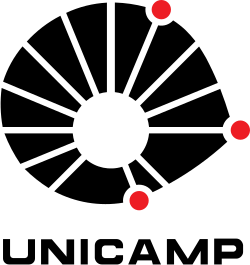
\includegraphics[width=0.3\textwidth]{imgs/university.png}
        
        \vspace*{1.5cm}

        \LARGE{UNIVERSIDADE ESTADUAL DE\\ CAMPINAS}

        \vspace{0.7cm}

        \Large{Instituto de Matemática, Estatística e\\ Computação Científica}

        \vspace*{2cm}
        
        Thiago Maximo Pavão\\ \small Orientador: Prof. Dr. Lúcio Tunes dos Santos
        
        \vspace*{2cm}

        \Huge{PICME - Esquerda Volver!}

        \vfill
        
        \Large
        Campinas\\
        2022
        
    \end{center}
\end{titlepage}
\tableofcontents

\chapter*{Introdução}

Aqui está documentado tudo que foi visto, aprendido e explorado durante o desenvolvimento do projeto pelo período de um ano. O projeto se iniciou no segundo semestre de 2021, em meio à pandemia. Me interessei pelo projeto por sua proposta exótica de estudar um sistema númerico semelhante ao que utilizamos usualmente, porém com uma diferença que muda completamente a forma que diversos números são representados, gerando resultados muito intrigantes.

Tive uma reunião inicial online com o orientador do projeto, Prof. Dr. Lúcio Tunes dos Santos, onde foi decidido o assunto que daria inicio aos estudos: bases. Apesar de já ter tido contato com números em outras bases no ensino fundamental, decidi começar os estudos desde o princípio, estudando o funcionamento do nosso sistema numérico, como converter números entre diferentes bases, como realizar operações em outras bases e algumas bases particulares com propiedades especiais, também fui aconselhado a registrar meus estudos em \LaTeX, um sistema que nunca havia utilizado mas que fui capaz de aprender passo a passo até construir este documento completo.

Continuamos nos reunindo a cada duas semanas, a cada reunião eu tirava eventuais dúvidas e discutíamos o andamento do projeto. Após finalizar o estudo de bases, começei a ler sobre os números esquerdistas, aprendi seu funcionamento, como converter nossos números para este outro sistema e como realizar algumas operações com estes números. Também vi uma aplicação da fórmula de convergência de série geométrica para números neste sistema, algo inusitado e interessante. Todo este trabalho foi desenvolvido até dezembro de 2021.

Retomamos os estudos em março de 2022, com uma reunião presencial com todos os orientados pelo professor. O trabalho agora era aprender os números $p$-ádicos, um sistema semelhante ao esquerdista porém trocando da base dez para outras diversas. Continuamos nos reunindo presencialmente uma vez a cada 2 ou 3 semanas enquanto aprendia mais sobre os $p$-ádicos e relatava meu progresso aqui. Mais próximo do fim, desenvolvi um programa em Python para automatizar a procura por inteiros $p$-ádicos usando os métodos aprendidos durante o semestre.

As atividades desenvolvidas durante este primeiro semestre de 2022 portanto, se encontram no Capítulo 3 deste documento. Sempre há mais a explorar, apesar do fim do projeto, mais poderia ser desenvolvido no futuro, isto foi detalhado na última Seção do último Capítulo. 

\chapter{Nosso sistema numérico}
\label{chapter:secaoBases}

\section{Introdução}

Diversos métodos de registrar quantidades foram desenvolvidos ao longo da história da humanidade, no entanto um dos sistemas sobressaiu e agora faz parte do nosso cotidiano.

Esse sistema é chamado sistema numérico posicional, que leva esse nome devido a importância da ordem dos dígitos em um número. 

\begin{figure}[H]
    \centering
    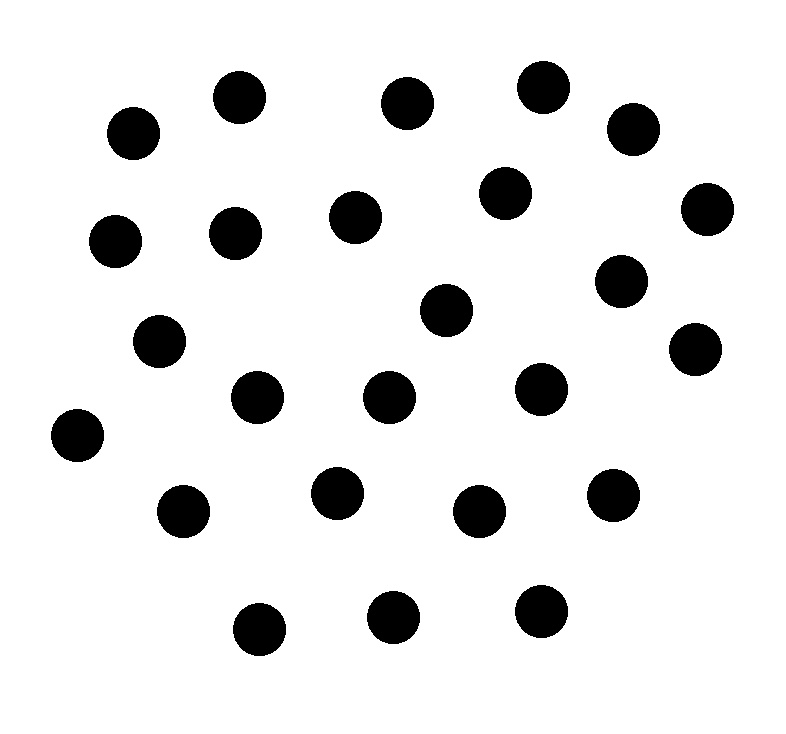
\includegraphics[width=0.27\textwidth]{imgs/pontos.png}
    \caption{Alguns pontos}
\end{figure}

Quantos pontos há na figura? Difícil saber sem contar um por um. Podemos fazer grupos de dez pontos enquanto há dez pontos completos para agrupar, fazendo isso obtemos:

\begin{figure}[H]
    \centering
    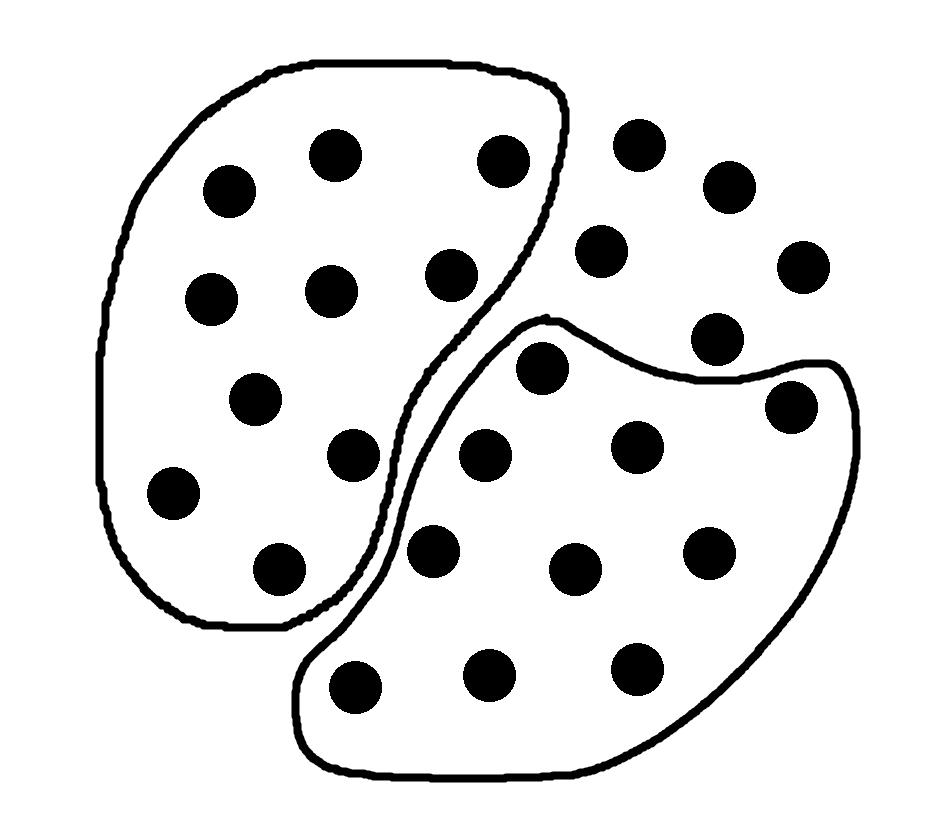
\includegraphics[width=0.27\textwidth]{imgs/pontosAgrupados.png}
    \caption{Pontos agrupados em dez}
\end{figure}

Disposto dessa forma, é fácil saber a quantidade. Temos dois grupos de dez e restam cinco pontos, logo temos 25 pontos. Se tivéssemos mais de cem pontos, seria necessário primeiro fazer grupos de cem, depois dez, e assim por diante para quantidades maiores.
E isso nos dá o funcionamento do sistema: Um número $A$ de $n+1$ algarismos representa a seguinte quantidade:

\begin{gather}
a_{n}a_{n-1} \ldots a_{1}a_{0} = \notag\\
a_{n} \times 10^{n} + a_{n-1} \times 10^{n-1} + \cdots + a_{1} \times 10 + a_{0} = \notag\\
\sum_{i=n}^{0}a_i \times 10^i
\end{gather}

Olhando para a quantidade de pontos encontrada temos

\begin{equation*}
25 = 2 \times 10 + 5 = 2 \times 10^1 + 5 \times 10^0
\end{equation*}

Que nos diz que existem dois grupos de dez e mais cinco pontos, se trocássemos a ordem dos dígitos teríamos o número 52, que nos diz que há 5 grupos de dez e mais dois, daí a importância da ordem dos algarismos.
\section{Os não inteiros}

Esse não é o sistema completo, pois com ele podemos representar apenas números inteiros, como a quantidade de pontos em uma imagem. Então como representar quantidades não inteiras, como a medida da barra a seguir em metros?

\begin{figure}[H]
    \centering
    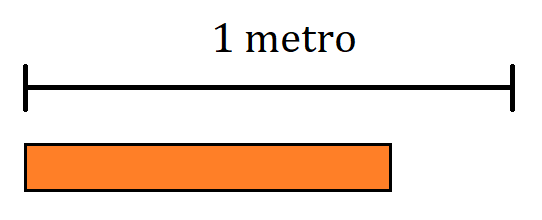
\includegraphics[width=0.5\textwidth]{imgs/barra_1.png}
    \caption{Barra a ser medida}
\end{figure}

Para realizar a medida, começamos dividindo o metro em dez partes, assim conseguimos visualizar quantos décimos de metro a barra mede:

\begin{figure}[H]
    \centering
    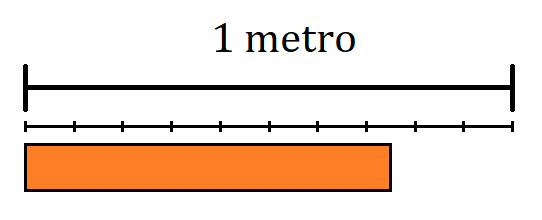
\includegraphics[width=0.5\textwidth]{imgs/barra_2.png}
    \caption{Barra com a divisão em décimos de metro}
\end{figure}

Agora é possível saber que a barra mede entre 7 e 8 décimos de metro, para obter mais precisão podemos dividir esse intervalo novamente em dez e explorar quantos centésimos a mais de 7 décimos de metro a barra mede. Fazendo a divisão e ampliando a figura temos:

\begin{figure}[H]
    \centering
    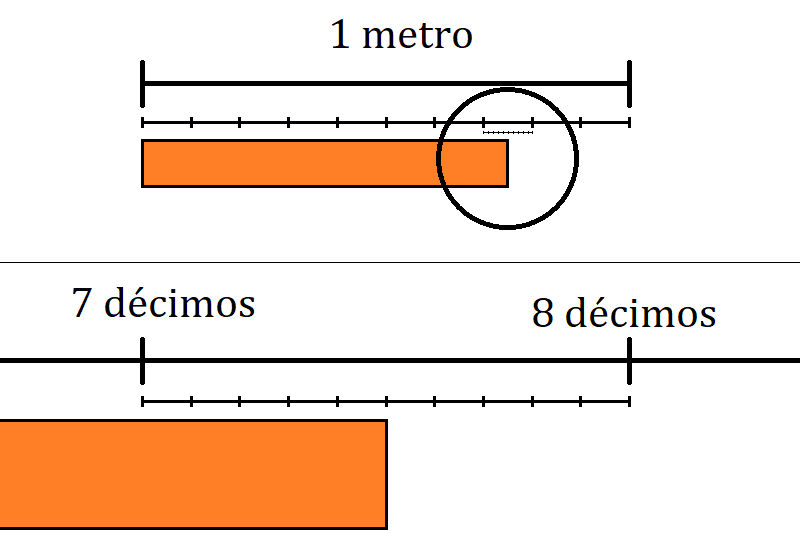
\includegraphics[width=0.5\textwidth]{imgs/barra_3.png}
    \caption{Barra com a divisão em centésimos de metro e ampliada}
\end{figure}

Note que com mais 5 centésimos de metro completa-se a medida da barra e portanto a barra mede 7 décimos + 5 centésimos de metro = 0,75 metros. Se não tivéssemos conseguido uma medida exata com centésimos, poderíamos dividir novamente em dez, visualizando milésimos e assim por diante.

Com isso podemos representar qualquer número real, que pode ter infinitos algarismos para a direita da vírgula. De forma geral, um número real $A$ qualquer representa a quantidade:

\begin{equation*}
a_n a_{n-1} \cdots a_1 a_0 , a_{-1} a_{-2} \cdots =
\end{equation*}
\begin{equation*}
a_{n} \times 10^{n} + a_{n-1} \times 10^{n-1} + \cdots + a_{1} \times 10^1 + a_{0} \times 10^0 + a_{-1} \times 10^{-1} + a_{-2} \times 10^{-2} + \cdots= \notag\\
\end{equation*}
\begin{equation}
\sum_{i=n}^{-\infty}a_i \times 10^i
\end{equation}

\section{Por que dez?}

Para contar o número de pontos da primeira figura formamos grupos de dez pontos, tornando fácil identificar a quantidade, também foi comentado que para quantidades maiores que cem pontos, seria necessário primeiro formar grupos de cem e assim por diante. Posteriormente, Para medir a barra, cada intervalo foi divido em dez repetidas vezes, nos dando décimos, centésimos, milésimos e assim por diante. Todos esses números são potências de dez, mas por que essa quantidade foi escolhida?

Essa quantidade é denominada base e é uma característica importantíssima do sistema, sem saber em que base um número foi escrito é impossível saber a quantidade que ele representa, escrevemos a base de um número como um subscrito, e por convenção um número sem subscrito está escrito na base dez.

Acredita-se que a quantidade de dedos nas mãos da maior parte das pessoas tenha sido o motivo da base dez ter sido padronizada, porém o que parece contraintuitivo é que essa escolha é arbitrária e não tem nenhuma vantagem sobre outras bases, a não ser a de que já estamos acostumados com ela.

Por exemplo, vamos contar novamente a quantidade de pontos da Figura 1, porém em base três.

Em vez de fazer grupos de dez, cem, mil... faremos grupos de potências de três: três, nove, vinte e sete... Note que não é possível formar um grupo de vinte e sete pontos e portanto devemos começar com grupos de nove e depois de três.

\begin{figure}[H]
    \centering
    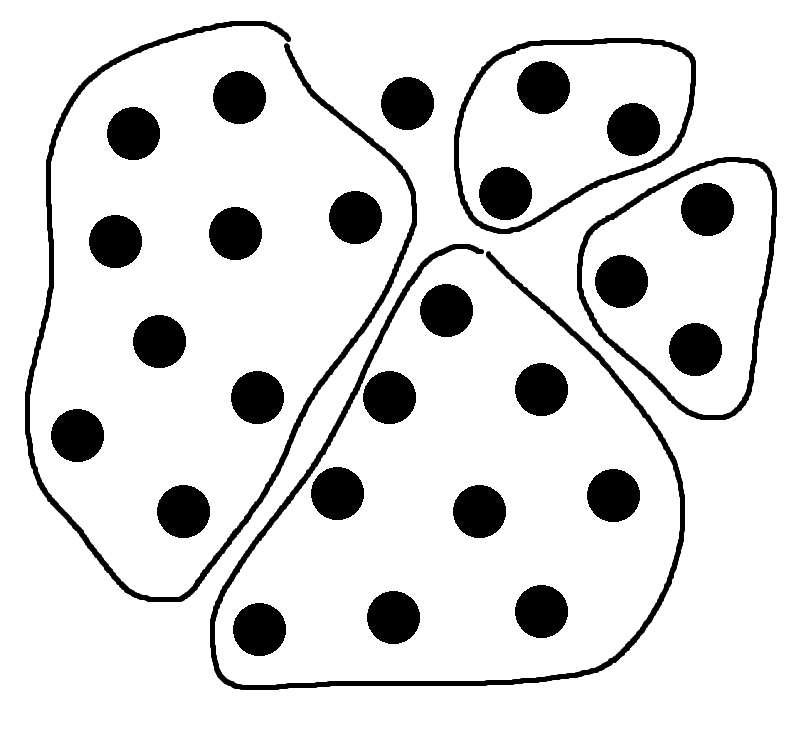
\includegraphics[width=0.3\textwidth]{imgs/pontosAgrupadosEm3.png}
    \caption{Pontos agrupados em potências de três}
\end{figure}

Temos dois grupos de nove, dois de três e resta um, portanto a quantidade de pontos é $221_3$. O mesmo poderia ser feito para medir a barra nessa base, ao invés de dividir o intervalo em dez partes, dividiríamos em três. Dessa maneira um número real qualquer $A$ em uma base $b$ representa a quantidade:

\begin{equation*}
a_n a_{n-1} \cdots a_1 a_0 , a_{-1} a_{-2} \cdots _{_b}=
\end{equation*}
\begin{equation*}
a_{n} \times b^{n} + a_{n-1} \times b^{n-1} + \cdots + a_{1} \times b^1 + a_{0} \times b^0 + a_{-1} \times b^{-1} + a_{-2} \times b^{-2} + \cdots=
\end{equation*}
\begin{equation} \label{eq:numeroReal}
\sum_{i=n}^{-\infty}a_i \times b^i
\end{equation}

Note que o número de algarismos diferentes necessários para escrever um número na base $b$ também é $b$, dado que $10_b = b^1 \times 1 + b^0 \times 0 = b$ e $10_b$ é o primeiro número de dois dígitos contando do 0. Para a base 3, por exemplo, temos os algarismos 0,1,2. Para uma base maior que dez, temos que adicionar símbolos, usualmente são adicionadas as letras maiúsculas. Para a base 16, por exemplo, podemos definir os algarismos como 0-9,A,B,C,D,E,F, onde:

\begin{equation*}
A_{16} = 10;\ B_{16} = 11;\ C_{16} = 12;\ D_{16} = 13;\ E_{16} = 14;\ F_{16} = 15
\end{equation*}

\section{Conversão entre bases}

Para converter um número de uma base $b$ qualquer para a base dez basta escrever o número na forma de somatório e fazer a conta, por exemplo, convertendo o número $A7F_{16}$ para base 10 temos:

\begin{align*}
A7F_{16} = A_{16} \times 16^2 & + & 7_{16} \times 16^1 & + & F_{16} \times 16^0 & = \\
10 \times 256 & + & 7 \times 16 & + & 15 \times 1 & = 2687
\end{align*}
\begin{equation*}
A7F_{16} = 2687
\end{equation*}

O processo inverso é mais complicado, para converter um número na base dez para uma base $b$ qualquer precisamos dividir o número pela base, e guardar o resto da divisão. Após isso dividimos o quociente pela base novamente e assim sucessivamente. O processo termina quando o quociente da divisão é um número menor que $b$, daí, para obter o número na nova base basta juntar o último quociente com os restos na ordem contrária à que eles foram obtidos. Confuso, porém com um exemplo fica fácil compreender:

Vamos converter 25 para base 3:

\[
    \begin{array}{rrr}
        25& |\underline{3}&   \\
         1&              8& |\underline{3}\\
          &              2&              2
    \end{array}
\]

Primeiro dividimos 25 por 3, obtendo resto 1 e quociente 8, este quociente é novamente divido por 3, que nos fornece resto 2 e quociente 2, o novo quociente: 2 é menor que 3 e portanto terminamos a divisão. Com isso basta pegar o quociente da última divisão e juntar com os restos da seguinte forma:

\[
    \begin{array}{rrr}
              25& |\underline{3}&               \\
     \circled{1}&              8& |\underline{3}\\
        \nwarrow&    \circled{2}&    \circled{2}\\
                &       \nwarrow&     \leftarrow
    \end{array}
\]

\begin{equation*}
\implies 25 = 221_3
\end{equation*}

Outro exemplo: Converter 42995 para base 16

\[
    \begin{array}{rrrr}
        42995& |\underline{16}&                &                \\
  \circled{3}&            2687& |\underline{16}&                \\
     \nwarrow&    \circled{15}&             167& |\underline{16}\\
             &        \nwarrow&     \circled{7}&    \circled{10}\\
             &                &        \nwarrow&      \leftarrow
    \end{array}
\]

$$10 = A_{16}; 15 = F_{16} \implies 42995 = A7F3_{16}$$

\section{Operações em outras bases}

Uma forma de realizar as operações básicas (soma, subtração, multiplicação e divisão) de números em outras bases seria converter os números para a base dez e fazer a conta, e depois converter o resultado para a outra base. Apesar de possível, essa forma seria muito ineficiente, dado que os algoritmos das operações podem ser reutilizados para fazer contas em outras bases de forma muito simples, apenas tomando alguns cuidados.

\subsection{Soma}

Assim como na base dez, para conseguir somar dois números quaisquer, basta saber o resultado da soma de dois dígitos na base dada. Por exemplo para a base 3:

\[
    \begin{array}{l l l}
        0_3 + 0_3 = 0_3  & 0_3 + 1_3 = 1_3  & 0_3 + 2_3 = 2_3 \\
        1_3 + 0_3 = 1_3  & 1_3 + 1_3 = 2_3  & 1_3 + 2_3 = 10_3\\
        2_3 + 0_3 = 2_3  & 2_3 + 1_3 = 10_3 & 2_3 + 2_3 = 11_3 
    \end{array}
\]

Esses resultados são obtidos contando-se na base nova, na base 3 os primeiros seis inteiros contando com o zero são:

$$0_3, 1_3, 2_3, 10_3, 11_3, 12_3, \ldots$$

Portanto para obter o resultado de $2_3 + 2_3$ na base 3 basta sair do dois na sequência e andar mais dois números, que nos dá $11_3$. Para somar dois números quaisquer basta fazer o mesmo procedimento, porém lembrando que a soma de dois dígitos é diferente da que estamos acostumados.

Por exemplo, somando $2120_3 + 2221_3$ temos:

\[
    \begin{array}{@{}B1}
           \carry 2\carry 120 \\
                    {} + 2221 \\ \hline
                        12111 \\
    \end{array}
\]

$$\implies 2120_3 + 2221_3 = 12111_3$$

Note que pode ser necessário fazer contas mais complicadas que dois dígitos sendo somados porém que no fundo são simples, por exemplo a conta feita na soma da última coluna: $1_3 + 2_3 + 2_3 = (1_3 + 2_3) + 2_3 = 10_3 + 2_3 = 12_3$

\subsection{Subtração}

Para a subtração basta tomar cuidado ao emprestar, quando não é possível fazer a subtração em uma coluna, ``emprestamos''  um da próxima coluna para a atual. Nessas situações, temos que tirar um número de um dígito de um de dois dígitos, o que pode causar certa confusão. Veja no exemplo a baixo:

Calcular $12111_3 - 2120_3$

\[
    \begin{array}{@{}B1}
                        12111 \\
                    {} - 2120 \\ \hline
                            1 \\
    \end{array}
\]

Não é possível tirar 2 de 1 então emprestamos da próxima coluna

\[
    \begin{array}{@{}B1}
                      12\carry[0]{\cancel 1} \carry11 \\
                    {} - 2120 \\ \hline
                            1 \\
    \end{array}
\]

Agora, precisamos fazer $11_3 - 2_3$, o resultado não é 9 pois não estamos trabalhando na base dez. Uma forma de fazer a conta é olhando a sequência dos primeiros números já colocada na página passada:

\begin{equation*}
0_3, 1_3, 2_3, 10_3, 11_3, 12_3, \ldots
\end{equation*}

Saímos do $11_3$ e voltamos 2, que por fim nos dá que $11_3 - 2_3 = 2_3$. Outra maneira seria converter momentaneamente para base dez, realizar a conta, e voltar para base três: $11_3 - 2_3 = (1 \times 3 + 1) - 2 = 4 - 2 = 2 = 2_3$. Completando a conta temos:

\[
    \begin{array}{@{}B1}
                      1\carry[1]{\cancel{2}}\carry[10]{\cancel 1} \carry11 \\
                    {} - 2120 \\ \hline
                         2221 \\
    \end{array}
\]

\begin{equation*}
\implies 12111_3 - 2120_3 = 2221_3
\end{equation*}

Outro problema que pode surgir é emprestar um de zero, conforme ocorre na seguinte conta:
Calcular $101_3 - 12_3$

\[
    \begin{array}{@{}B1}
                        101 \\
                    {} - 12 \\ \hline
    \end{array}
\]

$2_3>1_3$ portanto precisamos emprestar, como não é possível emprestar diretamente do 0, emprestamos do 1 da terceira casa

\[
    \begin{array}{@{}B1}
                        \cancel1 \carry 0 1 \\
                    {} - 12 \\ \hline
    \end{array}
\]

\[
    \begin{array}{@{}B1}
                        \cancel1 \carry[\cancel12]{\cancel0} \carry1 \\
                    {} - 12 \\ \hline
    \end{array}
\]

O problema ocorre ao emprestar pela segunda vez, temos que tirar um de $10_3$, que nos dá $2_3$ e não nove. Com isso basta terminar a conta

\[
    \begin{array}{@{}B1}
                        \cancel1 \carry[\cancel12]{\cancel0} \carry1 \\
                    {} - 12 \\ \hline
                         12
    \end{array}
\]

\begin{equation*}
    \implies 101_3 - 12_3 = 12_3
\end{equation*}

\subsection{Multiplicação}

Para a multiplicação, precisamos saber o resultado de multiplicações entre dígitos únicos, a tabuada. Na base dez, decoramos as tabuadas de 1 à 9, já na base três, precisamos decorar apenas de 1 e 2. Fazendo a tabela temos:

\begin{center}
    \begin{tabular}{ c|c|c } 
        $\times$ & 1 & 2 \\ 
        \hline
        1 & 1 & 2 \\ 
        \hline
        2 & 2 & 11 \\ 
    \end{tabular}
\end{center}

Com isso podemos fazer a multiplicação como usual, por exemplo, calculando $20_3 \times 12_3$

\[
    \begin{array}{@{}B1}
                              20\\
                    {} \times 12\\ \hline
                             110\\
                        {} + 20\hphantom{0}\\ \hline
                            1010
    \end{array}
\]

\begin{equation*}
\implies 20_3 \times 12_3 = 1010_3
\end{equation*}

\subsection{Divisão}

A divisão é a mais complicada, por envolver todas as outras três operações, mas também tem o mesmo funcionamento com o qual estamos acostumados.

Vamos calcular $1022_3 \div 12_3$:

\[
    \begin{array}{rr}
        1022& |\underline{12}\\
    \end{array}
\]

$1<12$ e $10<12$ portanto temos que agrupar os 3 primeiros algarismos do dividendo. Note que:

\[
    \begin{array}{@{}B1}
                             \carry12\\
                    {} \times 2\\ \hline
                             101 
    \end{array}
\]

\[
    \begin{array}{@{}B1}
                         102\\
                    {} - 101\\ \hline
                           1 
    \end{array}
\]

Logo o primeiro passo da divisão é:

\[
    \begin{array}{rr}
        1022& |\underline{12}\\
          12&               2\\
    \end{array}
\]

Por fim:

\[
    \begin{array}{rr}
        1022& |\underline{12}\\
          12&              21\\
           0&                \\
    \end{array}
\]

\begin{equation*}
\implies 1022_3 \div 12_3 = 21_3
\end{equation*}

\section{A base 3}

Como já dito, a base dez não tem nenhuma vantagem sobre qualquer outra, tirando a de que já estamos acostumados com ela. No entanto algumas bases podem ter algumas vantagens. Sabemos que quanto maior a base mais símbolos teremos e por consequência mais operações de soma e multiplicação entre algarismos precisam ser decoradas, porém com mais símbolos vem um crescimento mais lento na quantidade de dígitos necessária para representar um valor. O número 42995 por exemplo, escrito em base 16 é representado por $A7F3_{16}$, como visto na seção de conversão de bases. Nesse caso há apenas um algarismo de diferença, porém esse valor cresce cada vez mais para números maiores.

Com isso surge uma pergunta: qual base melhor equilibra o número de algarismos diferentes e o número de dígitos necessários para representar uma faixa de valores. A estratégia para encontrar a reposta é minimizar a multiplicação entre esses dois valores, com isso encontramos $e$ a constante de Euler. Como a base deve ser um número inteiro precisamos encontrar qual base (2 ou 3) minimiza a multiplicação, onde encontra-se 3.

Sabendo disso, faria sentido ter computadores que trabalhassem em base três, e não em binário como qualquer aparelho eletrônico de nosso cotidiano. Computadores ternários tem um grande ganho de eficiência por ganhar muito mais variação numérica para uma mesma quantidade de bits, no caso trits. Esses computadores já foram desenvolvidos mas foram descontinuados. Isso porque a tecnologia da época não permitia a criação de dispositivos capazes de armazenarem três estados diferentes de forma confiável. Hoje, toda a tecnologia desenvolvida para aparelhos binários torna difícil a conversão para dispositivos ternários, mesmo que estes agora possam ser desenvolvidos.

\section{A base 12}

Uma característica não comentada até o momento são as dízimas periódicas, qualquer número racional pode ser escrito como a divisão $p/q$ com $p$ e $q$ inteiros e coprimos. Sabe-se que essa divisão pode terminar ou repetir infinitamente, por exemplo, em base 10:

\begin{equation*}
\frac{1}{4} = 0,25,\ \frac{1}{3} = 0,33\ldots
\end{equation*}

Note que $1/4$ termina, enquanto $1/3$ é uma dízima periódica.

Para saber se uma fração terminará em sua forma decimal basta fatorar $q$, se $q$ é composto apenas por potências de 2 e 5 a fração termina, caso contrário, repete infinitamente, parcial ou completamente. Por exemplo:

\begin{equation*}
\frac{3}{60} = \frac{1}{20},\ 20 = 2^2 \times 5^1
\end{equation*}

Portanto $3/60$ deve terminar. Fazendo a conta temos que $3/60=0,05$.

O 2 e o 5 vêm da base escolhida, pois dez é divisível por 2 e por 5, 12 é divisível por 2, 3, 4 e 6 e portanto possui muito mais divisores. Por causa disso, diversos números que são dízimas periódicas em base dez terminam em base 12. $1/3 = 0,4_{12}$, $1/6 = 0,2_{12}$, $1/9 = 0,14_{12}$ por exemplo, logo, a base 12 também tem vantagens sobre a base dez e seria mais eficiente em nosso cotidiano.

Apesar de ter uma tabuada maior para decorar, a base 12 traz mais facilidade também nesse aspecto, pois são formados padrões que não se formam na base dez, e que facilitam a memorização.

Por exemplo, a tabuada do três em base 12 seria:

\begin{center}
    \begin{tabular}{ c|c|c|c|c|c|c|c|c|c|c|c|c|c } 
        $\times$ & 0 & 1 & 2 & 3 & 4 & 5 & 6 & 7 & 8 & 9 & X & E & 10\\ 
        \hline
        3 & 0 & 3 & 6 & 9 & 10 & 13 & 16 & 19 & 20 & 23 & 26 & 29 & 30\\ 
    \end{tabular}
\end{center}

Surge um padrão 0,3,6,9 na casa das unidades, algo que não ocorre na base dez e facilita a memorização.

\section{Formalizando}

Conclui-se que nosso sistema numérico é construído para representar qualquer quantidade real, para saber qual é essa quantidade é necessário saber em que base o número foi escrito. Com isso temos que qualquer número $A = \pm a_n a_{n-1} \cdots a_1 a_0 , a_{-1} a_{-2} \cdots _{_b}$ representa a quantidade dada pela Equação \ref{eq:numeroReal}, copiada aqui:

\begin{equation}\label{eq:numeroReal2}
    \pm a_n a_{n-1} \cdots a_1 a_0 , a_{-1} a_{-2} \cdots _{_b} = \pm \sum_{i=n}^{-\infty}a_i \times b^i
\end{equation}

É interessante notar que nesse sistema, a representação de um número não é única, qualquer número que termine pode ser representado de duas formas, como exemplo, o 1 também pode ser escrito como $0,999\ldots$, veja:

\begin{equation*}
    x=0,999\ldots \implies 10x=9,999\ldots
\end{equation*}
\begin{align*}
    10x - x & = 9,999 \ldots - 0,999 \ldots                 \\
    9x & = 9,\cancel{999 \ldots} - 0,\cancel{999 \ldots}    \\
    9x & = 9                                                \\
    x & = 1
\end{align*}
\begin{equation*}
\implies 0,999\ldots = 1
\end{equation*}

Outro ponto é que os algoritmos de operações básicas, com exceção ao da divisão, funcionam da direita para a esquerda, isso é um problema quando é necessário fazer operações entre números com representação infinita para a direita, pois não há onde começar. Veja o exemplo:

Qual o resultado de 1,812 794 64... + 3,187 205 35...? Somente com esses dados, é impossível definir qualquer algarismo do resultado, isso porque ele depende do valor das próximas casas do número dado. Por exemplo, se os números fossem 1,812 794 641 e 3,187 205 352 teríamos:

\[
    \begin{array}{@{}B4}
                    1,&812&794&641 \\
               {} + 3,&187&205&352 \\ \hline
                    4,&999&999&993 \\
    \end{array}
\]

Caso os números fossem 1,812 794 649 e 3,187 205 359 teríamos:

\[
    \begin{array}{@{}B4}
        \carry1,&\carry8\carry1\carry2&\carry7\carry9\carry4&\carry6\carry49 \\
               {} + 3,&187&205&359 \\ \hline
                    5,&000&000&008 \\
    \end{array}
\]

Sabemos que o resultado começa com 4,999 999 99 ou 5,000 000 00 porém para saber o resultado exato é necessário ter os dois números com todos seus algarismo definidos, e mesmo com eles, como fazer a conta? Começamos o algoritmo de soma pelo primeiro dígito antes da sequência infinita de zeros, em números que terminam, porém isso não pode ser feito em números que tenham infinitos algarismos diferentes de zero para a direita, números que existem em nosso sistema.

Esse problema também pode surgir na subtração e na multiplicação e é o motivo de pensarmos em um sistema que não sofra com ele.

\chapter{O sistema esquerdista}

\section{Saindo do padrão}

Como foi visto, em nosso sistema os números podem ter algarismos infinitamente para a direita, então podemos dizer que esse é um sistema direitista. Já no sistema esquerdista, os números podem ter algarismos infinitamente para a esquerda, por exemplo o número $\ldots 3333$, um número dessa forma não faz sentido em nosso sistema. Curiosamente, no sistema esquerdista, esse número é a representação de $-\frac{1}{3}$ veja:

\[
    \begin{array}{@{}B1}
                 \ldots3333 \\
                {} \times 3 \\ \hline
                 \ldots9999 \\
    \end{array}
\]

\[
    \begin{array}{@{}B1}
                \ldots\carry9\carry9\carry9 9 \\
                {} + 1 \\ \hline
                 \ldots0000 \\
    \end{array}
\]

\begin{equation*}
    \ldots0000 = 0
\end{equation*}

Nota-se que, $\ldots3333$ é um número tal que multiplicado por 3 e somado 1 ao resultado obtemos 0, assim como $-1/3$, logo $-1/3=\ldots3333$. Nesse mesmo exemplo também é possível perceber que -1 no sistema esquerdista é representado por $\ldots999$, pois é o número que somado um nos dá zero.

Antes de seguir em frente, é importante notar que qualquer número inteiro não negativo, e números racionais que terminem tem a mesma representação nos dois sistemas, por exemplo:

\begin{equation*}
    \frac{5}{4}=1,25=\ldots0001,25=1,25000\ldots
\end{equation*}

Lembrando que números racionais terminam quando a fração em sua forma mais simplificada tem o denominador somente múltiplo de 2 e 5, na base 10. Dessa forma, podemos definir um número número esquerdista qualquer $A=\ldots a_2 a_1 a_0 , a_{-1} a_{-2} \ldots a_{-n}$ que pode ser escrito na forma de somatório como sendo:

\begin{equation}
    \ldots a_2 a_1 a_0 , a_{-1} a_{-2} \ldots a_{-n} = \sum_{i=-n}^{\infty}a_i \times 10^i
\end{equation}

Note que diferentemente da representação dos números do sistema direitista (Equação \ref{eq:numeroReal2}), não temos o sinal + ou - antes do número, isso será explicado mais a frente porém o fato de que $\ldots 999 = -1$ já nos dá uma dica para a razão.

\section{Operações}

\subsection{Soma e Multiplicação}

As operações de soma e multiplicação são iguais as usuais, com a exceção de que como todo número no sistema esquerdista obrigatoriamente tem uma terminação a direita, nunca teremos o problema de não ter onde começar a conta, algo que poderia acontecer no sistema usual. Veja alguns exemplos de soma e multiplicação entre números esquerdistas:

\bigskip

\begin{tabular*}{330pt}{c c}

\begin{minipage}{150pt}
% Primeira conta
\[
    \begin{array}{@{}B5}
        \ldots 1& 231& 231& \carry 2\carry 34,& \carry 56 \\
    {}       &    &    &              + 98,& 34 \\ \hline
        \ldots 1& 231& 231& 332,& 90 \\
    \end{array}
\]
\begin{equation*}
    \overline{123}4,56 + 98,34 = \overline{123}1 332,9
\end{equation*}
\end{minipage}

    &

\begin{minipage}{150pt}
% Segunda conta
\[
    \begin{array}{@{}B1}
            \ldots \carry0 \carry9 \carry0 91 \\
       {} + \ldots 90910 \\ \hline
            \ldots 00001 \\
    \end{array}
\]
\begin{equation*}
    \overline{09}1 + \overline{09}10 = \ldots 0001=1
\end{equation*}
\end{minipage}

\bigskip \bigskip \\

\begin{minipage}{150pt}
% Terceira conta
\[
    \begin{array}{@{}B1}
    \ldots \carry6 \carry6 \carry6 6 \\
    {} \times 2 \\ \hline
            \ldots 3332 \\
    \end{array}
\]
\begin{equation*}
    \overline{6} \times 2 = \overline{3}2
\end{equation*}
\end{minipage}

    &

\begin{minipage}{150pt}
% Quarta conta
\[
    \begin{array}{@{}B1}
    \ldots 63637 \\
    {} \times 11 \\ \hline
        \ldots    \carry 6 \carry 3 \carry 637\\
    {} + \ldots 3637\hphantom{0}\\ \hline
        \ldots 00007
    \end{array}
\]
\begin{equation*}
    \overline{63}7 \times 11 = 7
\end{equation*}
\end{minipage}

\end{tabular*}

\bigskip

Note que uma conta entre dois números que terminem, por exemplo $34 \times 56$, também seria uma conta entre números esquerdistas, visto que ambos os números seriam esquerdistas e direitistas, não foi feito nenhum exemplo desse tipo pois a conta seria exatamente a mesma com a qual estamos acostumados.

\subsection{Subtração}

A subtração é feita adicionando-se o inverso aditivo de um número, então, precisamos saber se existe o inverso aditivo de um número qualquer no sistema esquerdista. Já vimos que $\ldots 999 + 1 = 0$, e portanto, $\ldots 999$ é o inverso aditivo de 1. Também podemos ver que $\ldots 998$ é o inverso aditivo de 2:

\[
    \begin{array}{@{}B1}
                 \ldots\carry9\carry9\carry98 \\
                {} + 2 \\ \hline
                 \ldots0000 \\
    \end{array}
\]

De forma geral, um número $A=\ldots a_2 a_1 a_0 , a_{-1} a_{-2} \ldots a_{-n}$ tem o inverso aditivo $-A$ da seguinte forma: 

\begin{equation}\label{eq:invAditivoEsq}
    -A=\ldots (9 - a_2) (9 - a_1) (9 - a_0) , (9 - a_{-1}) (9 - a_{-2}) \ldots (10 - a_{-n}), \text{para } a_{-n} \neq 0
\end{equation}

Prova:

\[
    \begin{array}{@{}B9}
                \ldots& \carry a_2& \carry a_1& \carry a_0,& \carry a_{-1}& \carry a_{-2}& \ldots& \carry a_{-n+1} & a_{-n} \\
                {} + \ldots& (9 - a_2)& (9 - a_1)& (9 - a_0),& (9 - a_{-1})& (9 - a_{-2})& \ldots& (9 - a_{-n+1}) & (10 - a_{-n})\\ \hline
                 \ldots&0&0&0&0&0&\ldots&0&0 \\
    \end{array}
\]

\begin{equation*}
    \implies A + (-A) = \ldots 000,0\ldots0 = 0
\end{equation*}

Então, no sistema esquerdista, qualquer número tem um inverso aditivo que pode ser facilmente calculado. Para fazer uma conta de subtração, primeiro encontra-se o inverso aditivo do número que está subtraindo, depois basta somar os números. Por exemplo:

\bigskip
$87 - 103 = ?$
\begin{equation*}
    87 - 103 = 87 + (-103)
\end{equation*}

O inverso aditivo de 103 é encontrado pelo método já mostrado (Equação \ref{eq:invAditivoEsq}), temos que, para $A = 103 = \ldots000103$

\begin{equation*}
    -A = \ldots(9-0)(9-0)(9-0)(9-1)(9-0)(10-3) = \ldots 999897
\end{equation*}

Por fim:

\begin{equation*}
    87 - 103 = 87 + (-103) = 87 + \ldots 999897
\end{equation*}

\[
    \begin{array}{@{}B1}
                \ldots 999 \carry 8 \carry 9 7\\
                {} + 87 \\ \hline
                 \ldots99984 \\
    \end{array}
\]

\begin{equation*}
    \implies 87 - 103 = \ldots99984
\end{equation*}

\bigskip

\bigskip
$103 - 87 = ?$

Novamente pela Equação \ref{eq:invAditivoEsq}, temos que:

\begin{equation*}
    -87 = \ldots 99913
\end{equation*}

\[
    \begin{array}{@{}B1}
                \ldots \carry 9 \carry 9 913\\
                {} + 103 \\ \hline
                 \ldots00016 \\
    \end{array}
\]

\begin{equation*}
    \implies 103 - 87 = 16
\end{equation*}

Note que neste caso não faz sentido encontrar o inverso aditivo de 87, visto que o resultado da subtração obtido pelo algoritmo usual de subtração nos daria um número do sistema esquerdista, no caso, 16. 

Na realidade, é possível encontrar o resultado de qualquer subtração sem encontrar o inverso aditivo, visto que podemos `emprestar' um da sequência infinita de zeros. Por exemplo, a conta 87 - 103 poderia ter sido realizada da seguinte forma:

\[
    \begin{array}{@{}B1}
                \ldots 00087\\
                {} - 103 \\ \hline
                84
    \end{array}
\]
Não é possível tirar 1 de 0 então emprestamos:
\[
    \begin{array}{@{}B1}
                \ldots \carry[9]{\cancel{0}} \carry[9]{\cancel{0}} \carry 0 87\\
                {} - 103 \\ \hline
                \ldots 99984
    \end{array}
\]

Por fim, também podemos encontrar o inverso aditivo de números com dízima, por exemplo:

\bigskip
$A = \ldots76767630, -A = ?$

Novamente pela Equação \ref{eq:invAditivoEsq}, temos que:
\begin{equation*}
    -A = \ldots(9-7)(9-6)(9-7)(9-6)(10-3)0 = \ldots 232370
\end{equation*}



\subsection{Divisão}

Da mesma forma que com a subtração, a divisão é dada pela multiplicação pelo inverso, então precisamos saber se um número esquerdista $q$ tem um inverso $1/q$. Lembrando que frações que terminam em nosso sistema usual tem o mesmo resultado no sistema esquerdista, por exemplo $1/4 = 0,25$ em ambos os sistemas, pois todos os números envolvidos são esquerdistas e direitistas.

É possível encontrar o inverso multiplicativo de um número realizando o algoritmo de divisão longa que já sabemos, porém com a diferença que a conta é feita da direita para a esquerda, usando o operador módulo.

\fbox{\begin{minipage}{300pt}

\textbf{O operador módulo}\\

O operador módulo nos da o resto da divisão de um número por outro. Por exemplo, $5\ \modulo 3 = 2$, esse operador também pode ser usado da seguinte forma:

\begin{equation}
    a \equiv b \ (\modulo c)
\end{equation}

Uma expressão como essa nos diz que o resto da divisão de $a$ por $c$ e de $b$ por $c$ são iguais, e portanto, $a-b$ é divisível por $c$. Por exemplo: $19 \equiv 3 \ (\modulo 8)$ e $19-3 = 16$ é divisível por 8.

\bigskip
Expressões desse tipo são essenciais para o algoritimo de longa divisão de números esquerdistas, como será visto em seguida.
\end{minipage}
}

\bigskip

Para encontrar o inverso de 3, $\dfrac{1}{3}$, fazemos a conta da seguinte forma:

\[
    \begin{array}{rr}
        \ldots 0001& |\underline{3}
    \end{array}
\]

O algarismo mais a direita do quociente é dado por $3a \equiv 1 \ (\modulo 10)$, em outras palavras, queremos que o dígito das unidades da multiplicação de a pelo divisor seja igual ao dígito das unidades do dividendo. Temos que $a=7$ então:

\[
    \begin{array}{rr}
        \ldots 0001& |\underline{3}\\
        \underline{-21}&             7
    \end{array}
\]

\bigskip

\[
    \begin{array}{@{}B1}
                \ldots \carry[9]{\cancel{0}} \carry[9]{\cancel{0}} \carry 0 1\\
                {} - 21 \\ \hline
                \ldots 99980
    \end{array}
\]

\bigskip

\[
    \begin{array}{rr}
        \ldots 0001& |\underline{3}\\
        \underline{-21}&             7\\
        \ldots 9998 \hphantom{1}&
    \end{array}
\]

O próximo dígito será dado por $3a \equiv 8 \ (\modulo 10),\ a=6$.

\[
    \begin{array}{rr}
        \ldots 0001& |\underline{\hphantom{6}3}\\
                \underline{-21}&             67\\
        \ldots 9998\hphantom{1}& \\
                \underline{-18}\hphantom{1}& \\
        \ldots 9998\hphantom{81}&
    \end{array}
\]

Como o resto se repetiu, não precisamos continuar a divisão. Temos que:

\[
    \begin{array}{rr}
        \ldots 0001& |\underline{\hphantom{\ldots 66}3}\\
                \underline{-21}&             \ldots 667\\
        \ldots 9998\hphantom{1}& \\
        \underline{-18}\hphantom{1}& \\
        \ldots 9998\hphantom{81}&
    \end{array}
\]

E portanto $\dfrac{1}{3} = \ldots 667$

\bigskip

Com o valor de um terço podemos obter facilmente múltiplos dele, como 2/3, 4/3, 5/3 e outras frações que sejam da forma $1/(3\times 2^n 5^m), \ n,m \in \mathbb{Z}^+$, por exemplo 1/6 e 1/15, da seguinte forma:

\bigskip

\begin{tabular*}{330pt}{c c}

\begin{minipage}{150pt}
% Primeira conta
\[
    \begin{array}{@{}B1}
                \ldots \carry 6 \carry 6 \carry 6 7\\
                {} \times 2 \\ \hline
                \ldots 3334
    \end{array}
\]

\begin{equation*}
    \implies \frac{2}{3} = 2 \times \frac{1}{3} = \overline3 4
\end{equation*}
\end{minipage}

    &

\begin{minipage}{150pt}
% Segunda conta
\[
    \begin{array}{@{}B1}
                \ldots \carry[3] 6 \carry[3] 6 \carry[3] 6 7\\
                {} \times 0,5 \\ \hline
                \ldots 333,5
    \end{array}
\]

\begin{equation*}
    \implies \frac{1}{6} = \frac{1}{2} \times \frac{1}{3} = \overline3,5
\end{equation*}
\end{minipage}

\end{tabular*}

\bigskip

O processo de longa divisão pode ser feito para encontrar o valor de $1/7=\overline{285714}3$, com ele podemos encontrar o valor de $-1/7=\overline{142857}$ que tem uma grande semelhança com o valor de $1/7$ no sistema direitista, $1/7=0,\overline{142857}$. Isso ocorre pois

\begin{equation*}
    7 \times \frac{1}{7} = 7 \times 0,\overline{142857} = 0,\overline{999999} = 1
\end{equation*}

no sistema direitista, e

\begin{equation*}
    7 \times \left( -\frac{1}{7} \right) = 7 \times \overline{142857} = \overline{999999} = -1
\end{equation*}

no sistema esquerdista. O mesmo ocorre para outros valores de $1/q$ se $q$ for coprimo com 10, então podemos enunciar o seguinte teorema:

\begin{theorem}
    Se $q$ e 10 forem coprimos, no sistema direitista $1/q = 0,\overline{b_1 \ldots b_k}$ se, e somente se, no sistema esquerdista $-1/q = \overline{b_1 \ldots b_k}$.
\end{theorem}

Prova: Ambas as equações só são corretas caso $q \times b_1 \ldots b_k = \underbrace{9 \ldots 9}_{k\text{ noves}}$

Podemos usar esse teorema para transformar dízimas do sistema direitista em dízimas do sistema esquerdista de forma simples. Veja:

\bigskip

Qual é a representação de $0,\overline{567}$ no sistema esquerdista?

\bigskip

Uma opção seria descobrir a fração que tem como resultado $0,\overline{567}$:

\begin{equation*}
    x = 0,\overline{567} \implies 1000x = 567,\overline{567}
\end{equation*}
\begin{equation*}
    1000x - x = 567,\cancel{\overline{567}} - 0,\cancel{\overline{567}} = 567
\end{equation*}
\begin{equation*}
    \implies x = \frac{567}{999} = 0,\overline{567} 
\end{equation*}

E realizar a divisão:

\[
    \begin{array}{rr}
        \ldots 00567& |\underline{\hphantom{0}999}\\
        \underline{-2997}&           \overline{243}3\\
        \ldots 99757\hphantom{1}&           \\
        \underline{-2997}\hphantom{1}&      \\
        \ldots 99676\hphantom{22}&          \\
        \underline{-3996}\hphantom{22}&     \\
        \ldots 99568\hphantom{333}&         \\
        \underline{-1998}\hphantom{333}&    \\
        \ldots 99757\hphantom{4444}&
    \end{array}
\]

\begin{equation*}
\implies 0,\overline{567} = \overline{243}3
\end{equation*}

\bigskip

Uma forma mais simples é obter o valor a partir do Teorema 1, da seguinte forma:

\begin{equation*}
    a = 0,\overline{567} \implies -a = \overline{567}
\end{equation*}

Usa-se o Teorema 1 para obter a representação do oposto do valor desejado no sistema esquerdista, agora, basta obter o inverso aditivo de $-a$ pela Equação \ref{eq:invAditivoEsq}, e portanto:

\begin{equation*}
    -(-a) = \ldots(9-5)(9-6)(9-7)(9-5)(9-6)(10-7) = \overline{243}3
\end{equation*}

\bigskip

\begin{equation*}
\implies 0,\overline{567} = \overline{243}3
\end{equation*}

Para números mais complexos, basta separar a dízima e realizar o processo, por exemplo:

\bigskip

Qual a representação de $12,34\overline{567}$ no sistema esquerdista?

\begin{equation*}
    12,34\overline{567} = 12,34 + 0,00\overline{567} = 12,34 + 0,\overline{567} \times 10^{-2}
\end{equation*}

Como já visto, $0,\overline{567} = \overline{243}3$, logo:

\begin{equation*}
     = 12,34 + \overline{243}3 \times 10^{-2} = 12,34 + \ldots24324,33
\end{equation*}

\[
    \begin{array}{@{}B1}
                \ldots 24324,33\\
                {} + 12,34 \\ \hline
                \ldots 24336,67
    \end{array}
\]

\begin{equation*}
    \implies 12,34\overline{567} = \overline{243}36,67
\end{equation*}

E dessa forma, qualquer número racional do sistema direitista pode ser escrito no sistema esquerdista.

\begin{theorem}
    Todo número no sistema esquerdista com uma dízima periódica pertence aos racionais
\end{theorem}

Prova:

\begin{equation*}
    \text{Seja }x = \overline{a_{k} \ldots a_1} \implies 10^kx=\overline{a_{k} \ldots a_1}\underbrace{0 \ldots 0}_{k\text{ zeros}}
\end{equation*}

\begin{equation*}
    x - 10^k x = \cancel{\overline{a_{k} \ldots a_1}} a_{k} \ldots a_1 - \cancel{\overline{a_{k} \ldots a_1}} 0 \ldots 0 = a_{k} \ldots a_1
\end{equation*}

\begin{equation}
    x = \frac{a_{k} \ldots a_1}{-\underbrace{9 \ldots 9}_{k\text{ noves}}}
\end{equation}

E portanto, $x$ é racional. Qualquer outro número racional pode ser escrito como a soma de um racional que termine e uma dízima da forma $\overline{a_{k} \ldots a_1}$ multiplicada por uma potência de 10, de forma similar ao que foi feito para encontrar $12,34\overline{567}$ no sistema esquerdista.

\section{Convergência de série geométrica}

Sabemos que a soma de todos os elemento de uma progressão geométrica de primeiro termo $a$ e razão $r$ converge para o valor:

\begin{equation}
    a + ar + ar^2 + \cdots = \frac{a}{1-r} \text{, para } |r| < 1
\end{equation}

No entanto, se ignorarmos a restrição de convergência, podemos usar a fórmula para encontrar a fração que tem como resultado um número esquerdista com dízima. Veja os exemplos:

\bigskip

\Ovalbox{\begin{minipage}{300pt}
\begin{equation*}
    \overline{567} = 567 + 567 \times 10^3 + 567 \times 10^6 + \cdots = \frac{567}{1 - 10^3} = -\frac{567}{999}
\end{equation*}

\begin{equation*}
    \therefore \overline{567} = -\frac{567}{999}
\end{equation*}

\smallskip

\end{minipage}}

\bigskip

\Ovalbox{\begin{minipage}{300pt}

\smallskip

\begin{equation*}
    \overline{243}3 = \overline{243} \times 10 + 3
\end{equation*}

\begin{equation*}
    \overline{243} = 243 + 243 \times 10^3 + 243 \times 10^6 + \cdots = \frac{243}{1 - 10^3} = -\frac{243}{999}
\end{equation*}


\begin{equation*}
    \implies \overline{243} \times 10 + 3 = -\frac{243}{999} \times 10 + 3 = -\frac{2430}{999} + 3 = \frac{567}{999}
\end{equation*}

\begin{equation*}
    \therefore \overline{243}3 =  \frac{567}{999}
\end{equation*}

\smallskip

\end{minipage}}

\bigskip

\Ovalbox{\begin{minipage}{300pt}

\smallskip

\begin{equation*}
    \overline{243}36,67 = \overline{243} \times 10^2 + 36,67
\end{equation*}

\begin{equation*}
    = -\frac{243}{999} \times 10^2 + 36,67 = -\frac{24.300}{999} + \frac{3667}{100} = \frac{45679}{3700}
\end{equation*}

\begin{equation*}
    \therefore \overline{243}36,67 =  \frac{45679}{3700} = 12,34\overline{567}
\end{equation*}

\smallskip

\end{minipage}}

% ========================================================== Números p-ádicos =================================================================

\chapter{Os números $p$-ádicos}

Apesar de ter um funcionamento interessante, os números esquerdistas não têm aplicação em outras áreas da matemática, entretanto, os números $p$-ádicos são bastante utilizados e se assemelham aos esquerdistas em diversos pontos. O $p$ em $p$-ádico se refere à um numero primo e indica a base do número, os números esquerdistas foram trabalhados inteiramente em base dez, um número não primo, isso gera problemas como divisores de zero e unidades, o que faz com que os números esquerdistas não formem um corpo. O uso exclusivo de números primos como base faz com que os p-ádicos não sofram desse problema, o que será provado à frente.

Um inteiro $p$-ádico é denotado e definido como
\begin{equation}
    \padc{\ldots, a_2, a_1, a_0}{p} = a_0 + a_1 \cdot p + a_2 \cdot p^2 + \cdots
\end{equation}

Onde $0 \leq a_i < p$ para todo $i \geq 0$.

Note que essa notação equivale à utilizada para um número esquerdista na forma $\ldots a_2 a_1 a_0$, e é vantajosa pois possibilita escrever números em bases maiores que dez sem a necessidade de designar novos símbolos para representar quantidades maiores que nove, dado que $a_i$ não precisa ser um dígito.

\section{Operações básicas} % --------- OPERAÇÕES ---------

Antes de estudar como encontrar a representação de números de nosso sistema no sistema dos $p$-ádicos é utíl aprender como somar e multiplicar inteiros $p$-ádicos, dado que com esse conhecimento poderemos realizar contas com os números que encontrarmos. As operações se dão da mesma forma que foi vista para os números esquerdistas, que por sua vez é análoga ao método que utilizamos em nosso sistema usual, a maior dificuldade vem do fato de estarmos fazendo contas em outras bases, essas operações podem ser feitas utilizando os métodos vistos no Capítulo \ref{chapter:secaoBases} porém isso pode ser simplificado utilizando um truque que será visto.

\subsection{Soma} % ------- SOMA -------

A soma é feita dígito a dígito, da direita para a esquerda, lembrando de realizar as operações na base $p$. Veja o exemplo:

\smallskip

\bigskip
\Ovalbox{\begin{minipage}{300pt}
\centerline{Determinar $\padc{1, 2, 0, 1, 1, 2}{3} + \padc{1, 0, 1, 2, 0}{3}$.}

\smallskip

Nesse caso $p=3$, e como já visto, para esta base, temos as seguintes somas entre dígitos:
\vspace*{-7pt}
\begin{equation*}
    1_3 + 1_3 = 2_3,\;\; 1_3 + 2_3 = 10_3,\;\; 2_3 + 2_3 = 11_3
\end{equation*}
Assim, basta realizar a soma
\vspace*{-7pt}
\[
    \begin{array}{@{}B1}
        [\; \carry1,\; 2,\; \carry0,\; \carry1,\; 1,\; 2\;]_3 \\
   {} + \padc{1,\; 0,\; 1,\; 2,\; 0 \;}{3} \\ \hline
        \padc{\; 2,\; 0,\; 1,\; 0,\; 0,\; 2 \;}{3}
    \end{array}
\]
\end{minipage}
}
\bigskip

Podemos utilizar a definição de um número $p$-ádico para encontrar a representação deste em nosso sistema, usando isso, podemos verificar se a soma do exemplo anterior está correta. Temos que

\vspace*{-15pt}
\begin{align*}
    [1, 2, 0, 1, 1, 2]_3 &=& 1 \cdot 3^5 + 2 \cdot 3^4 + 0 \cdot 3^3 + 1 \cdot 3^2 + 1 \cdot 3^1 + 2 \cdot 3^0 &=& 419 \\
    [1, 0, 1, 2, 0]_3    &=& 1 \cdot 3^4 + 0 \cdot 3^3 + 1 \cdot 3^2 + 2 \cdot 3^1 + 0 \cdot 3^0               &=& 96  \\
    [2, 0, 1, 0, 0, 2]_3 &=& 2 \cdot 3^5 + 0 \cdot 3^4 + 1 \cdot 3^3 + 0 \cdot 3^2 + 0 \cdot 3^1 + 2 \cdot 3^0 &=& 515
\end{align*}

Como esperado, $419 + 96 = 515$.

\smallskip

Não é prático lembrar das somas entre dígitos de cada base em que for necessário fazer uma conta, para evitar isso, podemos utilizar o truque já mencionado. Basta somar os dígitos, caso a soma seja menor que a base o dígito resultante é dado pela própria soma, caso contrário, o dígito resultante é dado pelo resto da divisão da soma pela base e o quociente é ``transportado" para o próximo dígito. 

Na realidade, o que esta sendo feito com esse truque é a conversão de qualquer número para a base em questão sempre que é necessário, desta forma elimina-se a necessidade de realizar somas em outras bases. Veja o seguinte exemplo, que utiliza esse método:

\bigskip
\Ovalbox{\begin{minipage}{300pt}
    \centerline{Determinar $\padc{1, 4, 2}{5} + \padc{4, 4, 1}{5} + \padc{3, 4, 3}{5}$.}
    
    \[
        \begin{array}{@{}B1}
        [\; \carry[2]1,\; \carry4,\; 2 \;]_5 \\
               \padc{\; 4,\; 4,\; 1 \;}{5} \\
          {} + \padc{\; 3,\; 4,\; 3 \;}{5} \\ \hline
          \padc{\; 2,\; 0,\; 3,\; 1 \;}{5}
        \end{array}
    \]

    \setlength{\parindent}{15pt}

    Para a primeira coluna temos $2 + 1 + 3 = 6 \geq 5$. Então, dividimos a soma pela base $6/5 = 1$, com resto 1. O resto fica no primeiro dígito do resultado e o quociente é levado para a próxima coluna.

    \smallskip

    Na segunda coluna temos $1 + 4 + 4 + 4 = 13 \geq 5$. Repetindo o processo temos $13/5 = 2$, resto 3. Novamente, o resto fica no resultado e o quociente é levado para a próxima coluna.

    \smallskip

    Para a última coluna o mesmo é feito, como não há mais números a esquerda o quociente é inserido como o quarto algarismo do resultado.
        
    \bigskip
\end{minipage}}

\bigskip
Também poderíamos ter números sem terminação à esquerda, em outras palavras, um número $p$-ádico tal que existe algum coeficiente $a_n \neq 0, n>N$, para todo $N \in \mathbb{N}$. Um exemplo de um número assim é o $\padc{\cdots,0,1,0,1,0,1}{2}$, somas que envolvem esse tipo de número são feitas da mesma forma, apenas tomando cuidado com qual padrão surgirá para o infinito. Veja o exemplo:

\bigskip
\Ovalbox{\begin{minipage}{300pt}
    \centerline{Determinar $\padc{\cdots, 0, 1, 0, 1}{2} + \padc{1, 1}{2}$.}
    
    \[
        \begin{array}{@{}B1}
                [\; \cdots,\; 0,\; 1,\; \carry0,\; \carry1,\; \carry0,\; 1 \;]_2 \\
                {} + \padc{\; 1,\; 1 \;}{2} \\ \hline
                \padc{\; \cdots,\; 0,\; 1,\; 0,\; 1,\; 1,\; 0,\; 0,\; 0 \;}{2}
        \end{array}
    \]
\end{minipage}}

\bigskip

Para evitar ambiguidade em relação ao que está se repetindo, será desenhada uma barra em cima da parte que se repete periodicamente, assim como fazemos em dízimas periódicas do nosso sistema. Escrevendo dessa forma a conta feita no exemplo acima, temos

\begin{equation*}
    \padc{\overline{0, 1}}{2} + \padc{1, 1}{2} = \padc{\overline{0, 1}, 1, 0, 0, 0}{2}
\end{equation*}

Como último exemplo, podemos também somar dois números sem terminação:

\bigskip
\Ovalbox{\begin{minipage}{300pt}
    \centerline{Determinar $\padc{\overline{10}}{13} + \padc{\overline{11}}{13}$.}
    
    \[
        \begin{array}{@{}B1}
                [\; \cdots ,\; \carry{10},\; \carry{10},\; 10 \;]_{13} \\
                {} + \padc{\; \cdots ,\; 11,\; 11,\; 11 \;}{13} \\ \hline
          \padc{\; \cdots,\; \hphantom{0}9,\; \hphantom{0}9,\; \hphantom{0}8 \;}{13}
        \end{array}
    \]

    \begin{equation*}
        \therefore \padc{\overline{10}}{13} + \padc{\overline{11}}{13} = \padc{\overline9,\; 8 \;}{13}
    \end{equation*}
\end{minipage}}

\bigskip
Note que não é possível obter facilmente a soma entre dois números em bases diferentes, por exemplo $\padc{\overline{10}, 5}{13} + \padc{1,2,0,3}{5}$, da mesma forma que não é trivial obter a soma entre dois números em bases diferentes em nosso sistema usual. Nos inteiros $p$-ádicos talvez seja necessário realizar a soma em uma terceira base, uma vez que existem números que não podem ser representados em qualquer base. Isso será visto com mais detalhe à frente.

\subsection{Multiplicação} % ------- MULTIPLICAÇÃO -------

A multiplicação é feita de maneira análoga à que estamos acostumados, mas como estaremos trabalhando em bases diferentes de dez é necessário utilizar o mesmo truque visto para a soma, dividir pela base e transportar o quociente. Veja os exemplos:

\bigskip
\Ovalbox{\begin{minipage}{300pt}
    \centerline{Determinar $\padc{2,1,2}{3} \times \padc{1, 2}{3}$.}
    
    \[
        \begin{array}{@{}B1}
                [\; 2,\; 1,\; 2 \;]_{3} \\
                {} \times \padc{\; 1,\; 2 \;}{3} \\ \hline
               1 \:\:\; 2 \:\:\; 0 \:\:\; 1 \; \hphantom{]_3}\; \\
               2 \:\:\; 1 \:\:\; 2 \:\: + \; \hphantom{]}\; \\ \hline
               \padc{\; 1,\; 1,\; 0,\; 2,\; 1 \;}{3}
        \end{array}
    \]

    Vamos por partes,

    Para encontrar a primeira linha da soma precisamos realizar a multiplicação lembrando de usar o truque, por exemplo na primeira coluna, $2 \times 2  = 4 \geq 3$, $4/3=1$, resto 1. Completando a operação, obtemos

    \[
        \begin{array}{@{}B1}
                [\; \carry2,\; \carry1,\; 2 \;]_{3} \\
                {} \times \padc{\; 2 \;}{3} \\ \hline
               1 \:\:\; 2 \:\:\; 0 \:\:\; 1 \; \hphantom{]_3}\;
        \end{array}
    \]

    
    A segunda multiplicação feita é por um, portanto basta copiar o número de cima. Por fim realiza-se a adição como foi visto anteriormente.

    \bigskip
\end{minipage}}

\bigskip
\Ovalbox{\begin{minipage}{300pt}
    \centerline{Determinar $\padc{\overline4}{5} \times \padc{3, 2}{5}$.}
    
    \[
        \begin{array}{@{}B1}
                [\; \cdots,\; 4,\; 4,\; 4 \;]_{5} \\
                {} \times \padc{\; 3,\; 2 \;}{5} \\ \hline
               \cdots \:\:\; 4 \:\:\; 4 \:\:\; 4 \:\:\; 3 \; \hphantom{]_3}\; \\
               \cdots \:\:\; 4 \:\:\; 4 \:\:\; 2 \:\: + \; \hphantom{]}\; \\ \hline
               \padc{\; \cdots,\; 4,\; 4,\; 1,\; 3 \;}{5}
        \end{array}
    \]

    Separando novamente, para cada dígito do segundo número, temos:

    \begin{center}
    \begin{tabular}{l | l}
        Para o primeiro & Para o segundo \\
        $
            \begin{array}{@{}B1}
                    [\; \cdots,\; \carry4,\; \carry4,\; 4 \;]_{5} \\
                    {} \times \padc{\; 2 \;}{5} \\ \hline
                    \cdots \:\:\; 4 \:\:\; 4 \:\:\; 4 \:\:\; 3 \; \hphantom{]_3}\;
            \end{array}
        $
        &
        $
            \begin{array}{@{}B1}
                    [\; \cdots,\; \carry[2]4,\; \carry[2]4,\; 4 \;]_{5} \\
                    {} \times \padc{\; 3 \;}{5} \\ \hline
                    \cdots \:\:\; 4 \:\:\; 4 \:\:\; 4 \:\:\; 2 \; \hphantom{]_3}\;
            \end{array}
        $
    \end{tabular}
    \end{center}

    Por fim, basta realizar a adição:

    \[
        \begin{array}{@{}B1}
               \cdots \:\:\; \carry4 \:\:\; \carry4 \:\:\; 4 \:\:\; 3 \; \hphantom{]_3}\; \\
               \cdots \:\:\; 4 \:\:\; 4 \:\:\; 2 \:\: + \; \hphantom{]}\; \\ \hline
               \padc{\; \cdots,\; 4,\; 4,\; 1,\; 3 \;}{5}
        \end{array}
    \]
\end{minipage}
}

\bigskip
Também podemos ter um caso com dois números sem terminação, esse caso é mais complexo, pois surge uma soma de infinitos termos. Como não é possível realiza-la, precisamos encontrar um padrão no resultado e generalizá-lo. Veja o exemplo:

\bigskip
\Ovalbox{\begin{minipage}{300pt}
    \centerline{Determinar $\padc{\overline6}{7} \times \padc{\overline6}{7}$.}
    
    \[
        \begin{array}{@{}B1}
                [\; \cdots,\; 6,\; 6,\; 6 \;]_{7} \\
                {} \times \padc{\; \cdots,\; 6,\; 6,\; 6 \;}{7} \\ \hline
               \cdots \:\:\; 6 \:\:\; 6 \:\:\; 6 \:\:\; 1 \; \hphantom{]_3}\; \\
               \cdots \:\:\; 6 \:\:\; 6 \:\:\; 1 \:\:\;   \;\hphantom{0]_3}\; \\
               \cdots \:\:\; 6 \:\:\; 1 \:\:\;\:\:\;\,\;   \;\hphantom{00]} \vspace{-5pt} \\
               \reflectbox{$\ddots$} \hphantom{00000000} + \hphantom{0]} \\ \hline
               \padc{\; \cdots,\; 0 ,\; 0,\; 0,\; 1 \;}{7}
        \end{array}
    \]

    Primeiramente, cada multiplicação será igual:

    \[
        \begin{array}{@{}B1}
                [\; \cdots,\; \carry[5]6,\; \carry[5]6,\; 6 \;]_{7} \\
                {} \times \padc{\; 6 \;}{7} \\ \hline
               \cdots \:\:\; 6 \:\:\; 6 \:\:\; 1 \; \hphantom{]_3}\; \\
        \end{array}
    \]
    
    Pois,\\
    Para a primeira coluna temos $6 \times 6 = 36 \geq 7$, $36/7 = 5$, resto 1.\\
    Para a segunda: $6 \times 6 + 5 = 41 \geq 7$, $41/7 = 5$, resto 6.\\
    Para as proxímas teremos uma repetição da segunda.

    \bigskip

    Na soma infinita, surge um padrão:
    
    \[
        \begin{array}{@{}B1}
               \cdots\:\:\; \carry[3]6 \:\:\; \carry[2]6 \:\:\; \carry6 \:\:\; 6 \:\:\; 1 \; \hphantom{]_3}\; \\
               \cdots\:\:\; 6 \:\:\; 6 \:\:\; 6 \:\:\; 1 \:\:\;   \;\hphantom{0]_3}\; \\
               \cdots\:\:\; 6 \:\:\; 6 \:\:\; 1 \:\:\;\:\:\;\,\;   \;\hphantom{00]}\\
               \cdots\:\:\; 6 \:\:\; 1 \:\:\;\:\:\;\:\:\;\,\;   \;\hphantom{000]} \vspace{-5pt} \\
               \reflectbox{$\ddots$} \,\;\; 1 \:\, \hphantom{0000000} + \hphantom{0]} \\ \hline
               \padc{\; \cdots,\; 0 ,\; 0 ,\; 0,\; 0,\; 1 \;}{3}
        \end{array}
    \]

    Note que a soma de cada coluna é exatamente um múltiplo de sete, o que faz com que o dígito do resultado seja zero, e o transporte feito é exatamente o necessário para continuar esse padrão.

    \begin{equation*}
        \therefore \padc{\overline6}{7} \times \padc{\overline6}{7} = \padc{1}{7}
    \end{equation*}
\end{minipage}}

\bigskip

Nesse exemplo temos algo interessante, encontramos um número nos $7$-ádicos que, quando multiplicado por ele mesmo resulta em um. Os únicos números com essa propriedade são $1$ e $-1$, logo $\padc{\cdots,6,6,6}{7} = -1$.

\section{Em busca de inteiros $p$-ádicos} % --------- ENCONTRANDO ---------

Até o momento sabemos que números $p$-ádicos são números esquerdistas em outras bases, então como encontrar a representação de um número inteiro qualquer nos $p$-ádicos? Isso pode ser feito a partir das soluções de uma sequência de congruências módulo $p^n$, parece complicado mas a ideia é muito simples.

Seja $x=\padc{\cdots,a_2,a_1,a_0}{p}$ um número $p$-ádico e $b$ um número inteiro do nosso sistema tal que $x=b$, nosso objetivo é determinar cada $a_i$, assim teremos encontrado a representação $p$-ádica de $b$. Temos que

\begin{equation}
    x = b \implies x \equiv b \ (\modulo y),
\end{equation}

para qualquer $y \in \mathbb{N} $.

Em particular, a congruência vale para $y = p^n$, $n > 0$. Para esses valores, algo interessante surge:

\smallskip

Para $n=1$:
\begin{align*}
    x \equiv b \ (\modulo p) & \implies & a_0 + a_1 \cdot p + a_2 \cdot p^2 + a_3 \cdot p^3 + \cdots \equiv b \ (\modulo p) &  \\
    & \implies & a_0 + p \cdot (a_1 + a_2 \cdot p^1 + a_3 \cdot p^2 + \cdots) \equiv b \ (\modulo p) & \\
    & \implies & a_0 \equiv b \ (\modulo p) &
\end{align*}

Seja $x_1 = a_0$ o primeiro elemento da nossa sequência, temos $x_1 = b \ (\modulo p)$.

\smallskip

Para $n=2$:
\begin{align*}
    x \equiv b \ (\modulo p^2) & \implies & a_0 + a_1 \cdot p + a_2 \cdot p^2 + a_3 \cdot p^3 + \cdots \equiv b \ (\modulo p^2) &\\
    & \implies & a_0 + a_1 \cdot p + p^2 \cdot (a_2 + a_3 \cdot p + \cdots) \equiv b \ (\modulo p^2) &\\
    & \implies & a_0 + a_1 \cdot p \equiv b \ (\modulo p^2) &
\end{align*}

Seja $x_2 = a_0 + a_1 \cdot p$, onde $x_2 = b \ (\modulo p^2)$

\smallskip

De forma geral, temos
\vspace{-4pt}
\begin{align}
    n &= 1: \; x \ (\modulo p^1) = x_1 = a_0                                                  &= b \ (\modulo p^1) \notag\\ 
    n &= 2: \; x \ (\modulo p^2) = x_2 = a_0 + a_1 \cdot p                                    &= b \ (\modulo p^2) \notag\\ 
    n &= 3: \; x \ (\modulo p^3) = x_3 = a_0 + a_1 \cdot p + a_2 \cdot p^2                    &= b \ (\modulo p^3) \notag\\ 
    n &= 4: \; x \ (\modulo p^4) = x_4 = a_0 + a_1 \cdot p + a_2 \cdot p^2 + a_3 \cdot p^3    &= b \ (\modulo p^4) \notag\\ 
    &\;\; \vdots & \label{sistcongru}
\end{align}

Também podemos relacionar cada elemento com o anterior na sequência:
\begin{equation} \label{eqSeq}
    x_{i+1} = x_{i} + a_i \cdot p^i \implies a_i = \dfrac{x_{i+1} - x_{i}}{p^i}, i \geq 1
\end{equation}

Concluindo, um número $p$-ádico $x=\padc{\cdots,a_2,a_1,a_0}{p} = b$, onde b é um número inteiro qualquer do nosso sistema pode ser encontrado a partir da sequência $(x_1,x_2,x_3,\cdots)$, sendo $x_n = b \ (\modulo p^n)$. Basta utilizar a Equação \ref{eqSeq} que permite obter cada coeficiente $a_i$ de $x$. Ou seja, a representação $p$-ádica de $b$.

\bigskip

\Ovalbox{\begin{minipage}{300pt}

    \centerline{Encontrar a representação de 10 nos 2-ádicos.}

    \bigskip

    Primeiro encontra-se a sequência a partir das congruências
    \begin{equation*}
        x \equiv 10 \ (\modulo 2^n)
    \end{equation*}\begin{align*}
        n &= 1: \; x \equiv 10  \ (\modulo 2) &\implies& x_1 = 10 \ (\modulo 2) = 0\\ 
        n &= 2: \; x \equiv 10  \ (\modulo 4) &\implies& x_2 = 10 \ (\modulo 4) = 2\\ 
        n &= 3: \; x \equiv 10  \ (\modulo 8) &\implies& x_3 = 10 \ (\modulo 8) = 2\\
        n &= 4: \; x \equiv 10  \ (\modulo 16) &\implies& x_4 = 10 \ (\modulo 16) = 10
    \end{align*}

    Para todo $n>4$ teremos o mesmo resultado que em $n=4$, $x_n = 10$. Assim, temos a sequência

    \begin{equation*}
        (0, 2, 2, 10, \ldots)
    \end{equation*}

    E portanto, obtém-se que
    \begin{equation*}
        \begin{aligned}[c]
        a_0 &= x_1 = 0 \\
        a_1 &= \dfrac{x_2-x_1}{2} = \dfrac{2-0}{2} = 1 \\
        a_2 &= \dfrac{x_3-x_2}{4} = \dfrac{2-2}{4} = 0
        \end{aligned}
        \hphantom{OO}\vline\hphantom{OO}
        \begin{aligned}[c]
        a_3 &= \dfrac{x_4-x_3}{8} = \dfrac{10-2}{8} = 1 \\
        a_4 &= \dfrac{x_5-x_4}{16} = \dfrac{10-10}{16} = 0 \\
            &\vdots
        \end{aligned}
    \end{equation*}

    Por fim, a representação 2-ádica de 10 é

    \begin{equation*}
        [\ldots,0,0,1,0,1,0]_2 = [1,0,1,0]_2
    \end{equation*}
    
\end{minipage}}

\bigskip    

Assim como a representação de inteiros não negativos esquerdistas e direitistas é a mesma, a representação de qualquer inteiro não negativo de nosso sistema usual será simplesmente a conversão do número para a base $p$ escolhida. Como foi possível ver no exemplo acima.

\subsection{Os negativos}

Qualquer inteiro negativo de nosso sistema tem representação infinita nos inteiros $p$-ádicos, isso será provado à frente. Como visto no último exemplo da Seção anterior, $-1 = \padc{\cdots,6,6,6}{7}$, também podemos chegar nesse resultado utilizando a sequência de congruências. Veja abaixo:

\Ovalbox{\begin{minipage}{300pt}

    \centerline{Encontrar a representação de $-1$ nos 7-ádicos.}

    \bigskip

    \begin{equation*}
        x \equiv -1 \ (\modulo 7^n)
    \end{equation*}
    
    \begin{gather*}
    \begin{align*}
    n &= 1: \; x \equiv -1  \ (\modulo 7) &\implies& x_1 = 6 \ (\modulo 9) = 6\\ 
    n &= 2: \; x \equiv -1  \ (\modulo 7^2) &\implies& x_2 = 48 \ (\modulo 49) = 48\\ 
    n &= 3: \; x \equiv -1  \ (\modulo 7^3) &\implies& x_3 = 342 \ (\modulo 343) = 342\\
    n &= 4: \; x \equiv -1  \ (\modulo 7^4) &\implies& x_4 = 2400 \ (\modulo 2401) = 2400
    \end{align*}\\
    \vdots
    \end{gather*}

    Assim, temos a sequência parcial

    \begin{equation*}
        (6, 48, 342, 2400, \ldots)
    \end{equation*}

    E portanto, obtém-se que
    \begin{equation*}
        \begin{aligned}[c]
        a_0 &= x_1 = 6 \\
        a_1 &= \dfrac{x_2-x_1}{7} = \dfrac{48-6}{7} = 6 \\
        a_2 &= \dfrac{x_3-x_2}{49} = \dfrac{342-48}{49} = 6
        \end{aligned}
        \hphantom{OO}\vline\hphantom{OO}
        \begin{aligned}[c]
        a_3 &= \dfrac{x_4-x_3}{343} = \dfrac{2400-342}{343} = 6 \\
            &\vdots
        \end{aligned}
    \end{equation*}

    Nota-se que o padrão continua e portanto, conclui-se que

    \begin{equation*}
        -1 = \padc{\cdots,6,6,6}{7}
    \end{equation*}
    
\end{minipage}}

\bigskip

Por fim, também podemos confirmar a validade desta representação de $-1$ ao somar $\padc{1}{7}$ à ela, temos

\[
\begin{array}{@{}B1}
        [\; \cdots,\; \carry6,\; \carry6,\; 6 \;]_7 \\
        {} + \padc{1}{7} \\ \hline
        \padc{\; \cdots,\; 0,\; 0,\; 0 \;}{7}
\end{array}
\]

Utilizando o mesmo método, podemos encontrar a representação $p$-ádica de $-1$ em qualquer base $p$. Cada termo $x_i$ da sequência é dado por

\begin{equation*}
    x \equiv -1  \ (\modulo p^i) \implies x_i = -1 \ (\modulo p^i) = p^i-1, i \geq 1\\ 
\end{equation*}

Logo, utilizando a Equação \ref{eqSeq}, temos os coeficientes

\begin{align*}
    & a_0 = x_1 = p^1-1 = p-1\\
    & a_i = \dfrac{x_{i+1}-x_{i}}{p^i} = \dfrac{p^{i+1}-1- \left(p^i-1 \right)}{p^i} = \dfrac{p \cdot p^i - p^i}{p^i} = p - 1, i \geq 1
\end{align*}

\begin{equation}
    \ovalbox{$-1 = \padc{\cdots,p-1,p-1,p-1}{p}$}
\end{equation}
Com a representação de $-1$ podemos obter o inverso adititivo (o oposto), de qualquer número $p$-àdico. Pela multiplicação

\[
\begin{array}{@{}B4}
        [\; \cdots,&\; a_2,&\; a_1,&\; a_0\;]_p \\
        {} \times [\; \cdots,&\; p-1,&\; p-1,&\; p-1 \;]_p \\ \hline
        [\; \cdots,&\; b_2,&\; b_1,&\; b_0\;]_p
\end{array}
\]

No entanto, é difícil determinar cada $b_i$ de forma geral por ela. Outra forma é escrever que a soma entre $a$ e $b$ seja zero, uma vez que é esta a definição de inverso aditivo. Fazendo dessa forma pode-se obter facilmente uma forma geral para $b = -a$, veja:

\[
\begin{array}{@{}B4}
        [\; \cdots,&\; a_2,&\; a_1,&\; a_0 \;]_p \\
        {} + [\; \cdots,&\; b_2,&\; b_1,&\; b_0 \;]_p \\ \hline
        [\; \cdots,&\; 0,&\; 0,&\; 0 \;]_p
\end{array}
\]

Temos que

\begin{equation}\label{eqSum}
    0 \leq a_i \leq p-1 \;\; \text{e} \;\; 0 \leq b_i \leq p-1 \implies  0 \leq a_i + b_i \leq 2 \cdot p - 2
\end{equation}

Para que a soma seja satisfeita, $a_0 + b_0 \ (\modulo p) = 0$, juntando isso à Equação \ref{eqSum} para $i=0$ obtém-se que $a_0 = b_0 = 0$ ou $a_0 + b_0 = p$. Como queremos encontrar o inverso aditivo de um número $a$ qualquer não existe certeza de que $a_0 = 0$, dessa forma escolhemos $b_0 = p - a_0$. Com $a_0 + b_0 = p$, ao realizar a soma, precisamos carregar um para a próxima coluna, então a soma nesta é dada por

\begin{equation*}
    a_1 + b_1 + 1 \ (\modulo p) = 0
\end{equation*}

Utilizando a restrição dada pela Equação \ref{eqSum}, temos

\begin{equation*}
    1 \leq a_1 + b_1 + 1 \leq 2 \cdot p - 1
\end{equation*}

Portanto, $ a_1 + b_1 + 1 = p \implies b_1 = p - 1 - a_1$. Essa mesma condição se repete para qualquer $i>1$.

\begin{equation}\label{eqOposite}
    \therefore -\padc{\cdots,a_2,a_1,a_0}{p} = \padc{\cdots,\; p-1-a_2,\; p-1-a_1,\; p-a_0}{p}
\end{equation}

\bigskip

\Ovalbox{\begin{minipage}{300pt}

    \centerline{Encontrar a representação de $-20$ nos 3-ádicos.}

    Já vimos que a representação de inteiros positivos nos $p$-ádicos é dada pela mudança de base, então
    
    \begin{equation*}
        20 = \padc{2,0,2}{3}
    \end{equation*}

    Agora, basta utilizar a Equação \ref{eqOposite}, para encontrar seu oposto.

    \begin{equation*}
        -20 = \padc{\cdots,2,2,0,2,1}{3}
    \end{equation*}

\end{minipage}}

\subsection{Os Racionais}

Novamente, nossa busca se dá pelo uso de congruências. Para encontrar a represenção $p$-ádica de $a/b$, onde $\mdc(a,b) = 1$ (fração irredutível), basta resolver o sistema dado por $b \cdot x \equiv a \ (\modulo p^n)$. Veja o exemplo:

\bigskip
\Ovalbox{\begin{minipage}{300pt}

    \centerline{Encontrar a representação de $\dfrac{2}{3}$ nos 5-ádicos.}

    \bigskip

    O sistema é dado por
    \begin{equation*}
        3 \cdot x \equiv 2 \ (\modulo 5^n)
    \end{equation*}

    \vspace*{-15pt}

    \begin{align*}
        & n = 1: \; 3 \cdot x \equiv 2  \ (\modulo 5)   & \implies & x_1 = 4    \\ 
        & n = 2: \; 3 \cdot x \equiv 2  \ (\modulo 5^2) & \implies & x_2 = 9    \\ 
        & n = 3: \; 3 \cdot x \equiv 2  \ (\modulo 5^3) & \implies & x_3 = 84   \\
        & n = 4: \; 3 \cdot x \equiv 2  \ (\modulo 5^4) & \implies & x_4 = 209  \\
        & n = 5: \; 3 \cdot x \equiv 2  \ (\modulo 5^5) & \implies & x_5 = 2084 
    \end{align*}
    \vspace*{-10pt}
    \begin{equation*}
    \vdots
    \end{equation*}

    E portanto, obtém-se que
    \begin{equation*}
        \begin{aligned}[c]
        a_0 &= x_1 = 4 \\
        a_1 &= \dfrac{x_2-x_1}{5} = \dfrac{9-4}{5} = 1 \\
        a_2 &= \dfrac{x_3-x_2}{25} = \dfrac{84-9}{25} = 3
        \end{aligned}
        \hphantom{OO}\vline\hphantom{OO}
        \begin{aligned}[c]
        a_3 &= \dfrac{x_4-x_3}{125} = \dfrac{209-84}{125} = 1 \\
        a_4 &= \dfrac{x_5-x_4}{625} = \dfrac{2084-209}{625} = 3 \\
            &\vdots
        \end{aligned}
    \end{equation*}

    Observando o padrão, conclui-se que

    \begin{equation*}
        \dfrac{2}{3} = \padc{\overline{1,3},4}{5}
    \end{equation*}

\end{minipage}}

\bigskip

Podemos conferir esse resultado multiplicando-o por três

\[
\begin{array}{@{}B1}
        [\; \cdots,\; \carry[2]1,\; \carry3,\; \carry[2]1,\; \carry3,\; \carry[2]1,\; 4 \;]_5 \\
        {} \times [\; 3 \;]_5 \\ \hline
        [\; \cdots,\; 0,\; 0,\; 0,\; 0,\; 0,\; 2 \;]_5
\end{array}
\]

Temos um número que multiplicado por três nos fornece dois, esse é certamente o $\frac{2}{3}$. Esse exemplo dá esperança de que todos os racionais do nosso sistema usual sejam inteiros $p$-ádicos, no entando isso não é verdade. Dado um $p$ fixo, existem racionais de nosso sistema que não tem representação nos $p$-ádicos, para este $p$. Por exemplo, veja o que ocorre ao tentarmos encontrar a representação de $\frac{1}{10}$ nos 5-ádicos. O sistema a ser resolvido é dado por

\begin{equation*}
    10 \cdot x \equiv 1 \ (\modulo 5^n)
\end{equation*}

Do lado esquerdo da congruência temos um múltiplo de 5: $2 \cdot 5 \cdot x$, e portanto, para $n=1$, seu resto na divisão por cinco é zero. Substituindo na congruência, temos 

\begin{equation*}
    10 \cdot x_1 \equiv 1 \ (\modulo 5) \implies 0 \equiv 1 \ (\modulo 5)
\end{equation*}
Absurdo!

\bigskip

Ou seja, não existe $x$ que satisfaça o sistema de congruências, e portanto não há representação de $1/10$ nos 5-ádicos. Isso ocorre sempre que $\mdc(b,p) \neq 1$, pois quando isso ocorre, o sistema $b \cdot x \equiv a \ (\modulo p^n)$ para $n=1$ é dado por:

\begin{align*}
    b \cdot x_1 & \equiv a \ (\modulo p)\\
            0 & \equiv a \ (\modulo p)
\end{align*}

\bigskip

Novamente obtemos um absurdo, conclui-se então que qualquer racional $a/b,\ \mdc(a,b) = 1$ tem representação $p$-ádica desde que $\mdc(b,p) = 1$, caso contrário, é necessário escolher outra base para representar o número.

\subsection{Os irracionais algébricos}

Qualquer número que seja solução de um polinômio de coeficientes inteiros é algébrico, exemplos destes são os inteiros positivos e negativos, e os racionais, que já vimos, além de muitos outros. Agora, vamos focar nos irracionais algébricos, a diferença desse conjunto para o dos irracionais é dada pelos números transcedentais, que incluem o número de Euler, Pi e outros. 

Esses números serão novamente encontrados por sistemas de congruências, e assim como ocorre com os racionais, nem todo irracional algébrico pode ser representado nos $p$-ádicos para um $p$ fixo, pode ser necessário trocar a base para ser possível representá-lo, como será visto. Iniciemos com um problema: 

\bigskip

\centerline{\textit{Encontrar a representação de $\mathit{\sqrt{3}}$ nos $p$-ádicos, na menor base possível.}}

\bigskip

O polinômio $f(x) = x^2 - 3$ tem como raiz $x = \sqrt{3}$, então o sistema de congrûencias nesse caso é dado por

\vspace*{-5pt}
\begin{equation*}
    x^2 \equiv 3 \ (\modulo p^n)
\end{equation*}

Queremos a menor base então começaremos em $p=2$:

\smallskip

Para $n=1$:

\vspace*{-5pt}
\begin{align*}
             & x_1^2 \equiv 3 \ (\modulo 2) \\
    \implies & x_1^2 \equiv 1 \ (\modulo 2) \\
    \implies & x_1 = 1
\end{align*}

Para $n=2$:

\begin{equation*}
    x_2^2 \equiv 3 \ (\modulo 4)
\end{equation*}

Sabemos da Equação \ref{eqSeq} que $x_2 = x_1 + a_1 \cdot p^1 = 1 + 2 \cdot a_1$, com $a_1 \in \left\lbrace 0,1 \right\rbrace$. No entanto, nenhuma das possibilidades satisfaz a congruência, e portanto, $\sqrt{3}$ não pode ser representado nos 2-ádicos. Considerando agora $p=3$, temos o sistema

\begin{equation*}
    x^2 \equiv 3 \ (\modulo 3^n)
\end{equation*}

Para $n=1$:

\begin{align*}
             & x_1^2 \equiv 3 \ (\modulo 3) \\
    \implies & x_1^2 \equiv 0 \ (\modulo 3) \\
    \implies & x_1 = 0
\end{align*}

Para $n=2$:

\begin{equation*}
    x_2^2 \equiv 3 \ (\modulo 9)
\end{equation*}

Novamente, pela Equação \ref{eqSeq}, temos $x_2 = x_1 + a_1 \cdot p^1 = 0 + 3 \cdot a_1$, com $a_1 \in \left\lbrace 0,1,2 \right\rbrace$. Assim, como para $n=2$, nenhuma das possibilidades de $x_2$ satisfaz a congruência, conclui-se que $\sqrt{3}$ não pode ser representado nos 3-ádicos. A próxima base possível é $p=5$, que nos dá o sistema

\begin{equation*}
    x^2 \equiv 3 \ (\modulo 5^n)
\end{equation*}

A partir de agora, não é preciso testar $n=2$, pois o lado direito da congruência não se altera.

Para $n=1$:

\begin{equation*}
    x_1^2 \equiv 3 \ (\modulo 5)
\end{equation*}

Sabemos que $x_1 = a_0 \in \left\lbrace 0,1,2,3,4 \right\rbrace$, podemos testar todas as possibilidades encontrando o conjunto de possíveis resíduos quadráticos, $x_1^2 \ (\modulo 5)$, temos que

\begin{align*}
             x_1                 &\in \left\lbrace 0,1,2,3,4 \right\rbrace\\
    \implies x_1^2               &\in \left\lbrace 0,1,4,9,16 \right\rbrace\\
    \implies x_1^2 \ (\modulo 5) &\in \left\lbrace 0,1,4,4,1 \right\rbrace = \left\lbrace 0,1,4 \right\rbrace
\end{align*}

Não existe $x_1$ tal que $x_1^2 \ (\modulo 5)=3$, logo também não há representação de $\sqrt{3}$ nos 5-ádicos. Para $p=7$, $n=1$ temos:

\begin{equation*}
    x_1^2 \equiv 3 \ (\modulo 7)
\end{equation*}

\begin{equation*}
    x_1 \in \left\lbrace 0,1,2,3,4,5,6 \right\rbrace \implies x_1^2 \ (\modulo 7) \in \left\lbrace 0,1,2,4 \right\rbrace
\end{equation*}

Sem sucesso novamente, testemos a próxima base, para $p=11$, $n=1$ obtém-se

\begin{equation*}
    x_1^2 \equiv 3 \ (\modulo 11)
\end{equation*}

\begin{equation*}
    x_1 \in \left\lbrace 0,1,\cdots,9,10 \right\rbrace \implies x_1^2 \ (\modulo 11) \in \left\lbrace 0,1,\circled{3},4,5,9 \right\rbrace
\end{equation*}

Finalmente, encontramos uma base em que a primeira congrûencia tem solução, agora resta resolver mais etapas do sistema para determinar alguns coeficientes do número. É interessante notar que $x_1^2 \ (\modulo 11) = 3$ é válido tanto para $x_1 = 5$ quanto para $x_1 = 6$, ou seja, teremos duas sequências que satisfazem a equação. Isso era esperado pois estamos considerando a equação $x^2 = 3$, e portanto iremos encontrar a representação de dois números: $\pm \sqrt{3}$.

Continuando primeiro para a sequência dada por $x_1 = 5$, temos

\bigskip
        
Para $n = 2$:
\begin{equation*}
    x_2^2 \equiv 3 \ (\modulo 11^2)
\end{equation*}

Substituindo $x_2 = 5 + 11 \cdot a_1$, para facilitar a resolução da congruência
\begin{align*}
    (5 + 11 \cdot a_1)^2 &\equiv 3 \ (\modulo 121) \\
    25 + 2 \cdot 5 \cdot 11 \cdot a_1 + 11^2 \cdot a_1^2 &\equiv 3 \ (\modulo 121) \\
    2 \cdot 5 \cdot 11 \cdot a_1 &\equiv -22 \ (\modulo 121) \\
    10 \cdot 11 \cdot a_1 &\equiv 99 \ (\modulo 121) \\
    10 \cdot 11 \cdot a_1 &\equiv 9 \cdot 11 \ (\modulo 11^2) \\
    10 \cdot a_1 &\equiv 9 \ (\modulo 11) \\
    \implies a_1 &= 2
\end{align*}

Com esse valor podemos encontrar o segundo termo da sequência, $x_2 = 5 + 11 \cdot 2 = 27$, já encontramos $a_1$, o segundo coeficiente da série de potências então não precisaremos utilizar a sequência $\left( x_0,x_1,x_2,\cdots \right)$ novamente para encontrar este coeficiente.

\bigskip
        
Para $n = 3$:
\begin{equation*}
    x_3^2 \equiv 3 \ (\modulo 11^3)
\end{equation*}

Novamente, $x_3 = x_2 + a_2 \cdot p^2 = 27 + 11^2 \cdot a_2$
\begin{align*}
    (27 + 11^2 \cdot a_2)^2 &\equiv 3 \ (\modulo 11^3) \\
    27^2 + 2 \cdot 27 \cdot 11^2 \cdot a_2 + 11^4 \cdot a_2^2 &\equiv 3 \ (\modulo 11^3) \\
    54 \cdot 11^2 \cdot a_2 + 11^3 \cdot 11 \cdot a_2^2 &\equiv 605 \ (\modulo 11^3) \\
    54 \cdot 11^2 \cdot a_2 &\equiv 5 \cdot 11^2 \ (\modulo 11^3) \\
    54 \cdot a_2 &\equiv 5 \ (\modulo 11) \\
    4 \cdot 11 \cdot a_2 + 10 \cdot a_2 &\equiv 5 \ (\modulo 11) \\
    10 \cdot a_2 &\equiv 5 \ (\modulo 11) \\
    \implies a_2 &= 6
\end{align*}

Esse processo pode ser seguido para encontrar mais coeficientes, parando aqui temos a série de potências parcial

\begin{equation*}
    x_a = 5 + 2 \cdot 11 + 6 \cdot 11^2 + \cdots
\end{equation*}

Que nos fornece o 11-ádico

\begin{equation*}
    x_a = \padc{\cdots,6,2,5}{11}
\end{equation*}

Podemos conferir que este satisfaz a equação $x^2 = 3$, veja:

\[
\begin{array}{@{}B1}
        [\; \cdots,\; 6,\; 2,\; 5 \;]_{11} \\
        \times \; [\; \cdots,\; 6,\; 2,\; 5 \;]_{11} \\ \hline
        \cdots\;\:\: 9\;\:\: 1\;\:\: 3 \;\hphantom{]_{11}}\\
        \cdots\;\:\: 1\;\:\: 4\:\: 10\;\;\:\: \;\hphantom{]_{11}}\\\vspace*{-3pt}
        \cdots\;\:\: 4\;\:\: 3\;\:\: 8\;\:\: \;\:\;+ \hphantom{]_{11}}\\
        \reflectbox{$\ddots$}\hphantom{000000} \;\:\: \;\hphantom{]_{11}}\\ \hline
        [\; \cdots,\; 0,\; 0,\; 3 \;]_{11}
\end{array}
\]

\bigskip

Ainda falta encontrar a segunda sequência que satisfaz o sistema de congruências, para esta, temos $x_1 = 6$ e é feito o mesmo processo:

\bigskip
        
Para $n = 2$:
\begin{equation*}
    x_2^2 \equiv 3 \ (\modulo 11^2)
\end{equation*}

Temos $x_2 = 6 + 11 \cdot a_1$
\begin{align*}
    (6 + 11 \cdot a_1)^2 &\equiv 3 \ (\modulo 121) \\
    36 + 2 \cdot 6 \cdot 11 \cdot a_1 + 11^2 \cdot a_1^2 &\equiv 3 \ (\modulo 121) \\
    2 \cdot 6 \cdot 11 \cdot a_1 &\equiv -33 \ (\modulo 121) \\
    12 \cdot 11 \cdot a_1 &\equiv 88 \ (\modulo 121) \\
    12 \cdot 11 \cdot a_1 &\equiv 8 \cdot 11 \ (\modulo 11^2) \\
    12 \cdot a_1 &\equiv 8 \ (\modulo 11) \\
    a_1 &\equiv 8 \ (\modulo 11) \\
    \implies a_1 &= 8
\end{align*}

Portanto, $x_2 = 6 + 11 \cdot 8 = 94$.

\bigskip
        
Para $n = 3$:
\begin{equation*}
    x_3^2 \equiv 3 \ (\modulo 11^3)
\end{equation*}

Novamente, $x_3 = x_2 + a_2 \cdot p^2 = 94 + 11^2 \cdot a_2$
\begin{align*}
    (94 + 11^2 \cdot a_2)^2 &\equiv 3 \ (\modulo 11^3) \\
    94^2 + 2 \cdot 94 \cdot 11^2 \cdot a_2 + 11^4 \cdot a_2^2 &\equiv 3 \ (\modulo 11^3) \\
    188 \cdot 11^2 \cdot a_2 + 11^3 \cdot 11 \cdot a_2^2 &\equiv 484 \ (\modulo 11^3) \\
    188 \cdot 11^2 \cdot a_2 &\equiv 4 \cdot 11^2 \ (\modulo 11^3) \\
    188 \cdot a_2 &\equiv 4 \ (\modulo 11) \\
    17 \cdot 11 \cdot a_2 + a_2 &\equiv 4 \ (\modulo 11) \\
    a_2 &\equiv 4 \ (\modulo 11) \\
    \implies a_2 &= 4
\end{align*}

Portanto, temos a série de potências

\begin{equation*}
    x_b = 6 + 8 \cdot 11 + 4 \cdot 11^2 + \cdots
\end{equation*}

Que nos fornece o 11-ádico

\begin{equation*}
    x_b = \padc{\cdots,4,8,6}{11}
\end{equation*}

Portanto, encontramos dois números $x_a = \padc{\cdots,6,2,5}{11}$ e $x_b = \padc{\cdots,4,8,6}{11}$ tais que elevados ao quadrado resultam em 3. Vale notar que $x_a + x_b = 0$ pois

\[
\begin{array}{@{}B1}
        [\; \cdots,\; \carry6,\; \carry2,\; 5 \;]_{11} \\
        + \; [\; \cdots,\; 4,\; 8,\; 6 \;]_{11} \\ \hline
        [\; \cdots,\; 0,\; 0,\; 0 \;]_{11}
\end{array}
\]

Então temos as representações de $\sqrt 3$ e $- \sqrt 3$.

Não era necessário resolver o sistema novamente para $x_1 = 6$, pois para cada $x_i$ encontrado na primeira sequência podemos concluir que $p-x_i$ também é solução. \textit{Prova:}

Seja $x$ um inteiro tal que $0 \leq x \leq p-1$, $a$ e $b$ inteiros positivos, tal que $a<b$. Se $x^2 \equiv a \ (\modulo b) \implies (b-x)^2 \equiv a \ (\modulo b)$, pois

\smallskip
\begin{align*}
    x^2 &\equiv a \ (\modulo b) \\
    b \cdot (b - 2 \cdot x) + x^2 &\equiv a \ (\modulo b) \\
    b^2 - 2 \cdot b \cdot x + x^2 &\equiv a \ (\modulo b) \\
    (b-x)^2 &\equiv a \ (\modulo b)
\end{align*}

Logo, no problema feito, com a sequência $(5,27,753,\cdots)$ já poderíamos obter a sequência $(11-5,11^2-27,11^3-753,\cdots) = (6,94,578,\cdots)$, que nos fornece $x_b$.

De forma geral, podemos querer resolver qualquer sistema da forma

\begin{equation}\label{eqQuadGeral}
    a \cdot x^2 + b \cdot x + c \equiv 0 \ (\modulo p^n) 
\end{equation}

\smallskip

para encontrar a representação $p$-ádica de $\dfrac{-b + \sqrt{b^2-4ac}}{2a}$ e $\dfrac{-b - \sqrt{b^2-4ac}}{2a}$.

\smallskip

Para isso basta resolver o sistema dado pela Equação \ref{eqQuadGeral}, porém, não é fácil resolvê-lo de maneira direta, podemos facilitar o processo com as seguintes manipulações:

\begin{align*}
    a \cdot x^2 + b \cdot x + c &= 4a^2 \cdot x^2 + 4ab \cdot x + 4ac \\
                                &= (2ax)^2 + 2 \cdot 2ax \cdot b + b^2 - b^2 + 4ac \\
                                &= (2ax+b)^2 - b^2 + 4ac
\end{align*}

Substituindo a relação encontrada na Equação \ref{eqQuadGeral}, temos

\begin{align*}
    (2ax+b)^2 - b^2 + 4ac &\equiv 0\hphantom{^2 - 4ac} \ (\modulo p^n) \\
    (2ax+b)^2             &\equiv b^2 - 4ac \ (\modulo p^n) 
\end{align*}

Seja $\alpha = 2ax+b$ e $\beta = b^2 - 4ac$, obtém-se o sistema:

\begin{equation}\label{eq:QuadSimplificada}
    \alpha^2 \equiv \beta \ (\modulo p^n) 
\end{equation}

Agora, basta resolver o sistema em alfa e posteriormente realizar a substituição para encontrar a sequência em $x$. Veja o processo com um exemplo: Encontrar a representação $p$-ádica do número de ouro, $\varphi$, na menor base em que ele seja representável.

\bigskip

O número de ouro é dado pela solução positiva da equação $x^2 - x - 1 = 0$, portanto, para encontrar a representação $p$-ádica dele, basta resolver o sistema dado por

\begin{equation*}
    x^2 - x - 1 \equiv 0 \ (\modulo p^n)
\end{equation*}

Que pode ser simplificado usando a Equação \ref{eq:QuadSimplificada}:

\begin{equation*}
    \alpha^2 \equiv 5 \ (\modulo p^n), \ \alpha = 2x-1
\end{equation*}

Ao realizar o mesmo processo feito para encontrar a menor base em que $\sqrt3$ é representável encontra-se que, neste caso, a menor base possível é $p=11$.

Resolvendo o sistema temos:

\bigskip

Para $n = 1$:

\begin{equation*}
    \alpha_1^2 \equiv 5 \ (\modulo 11) \implies \alpha_1 \equiv \pm 4 \ (\modulo 11)
\end{equation*}

\begin{equation*}
    \begin{aligned}[c]
        2 \cdot x_1 - 1 &\equiv 4 \ (\modulo 11)\\
        2 \cdot x_1 &\equiv 5 \ (\modulo 11)\\
        x'_1 &= 8
    \end{aligned}
    \hphantom{OO}\vline\hphantom{OO}
    \begin{aligned}[c]
        2 \cdot x_1 - 1 &\equiv -4 \ (\modulo 11)\\
        2 \cdot x_1 &\equiv 8 \ (\modulo 11)\\
        x''_1 &= 4
    \end{aligned}
\end{equation*}

Para $n = 2$:

\begin{equation*}
    \alpha_2^2 \equiv 5 \ (\modulo 11^2) \implies \alpha_2 \equiv \pm 48 \ (\modulo 11^2)
\end{equation*}

\begin{equation*}
    \begin{aligned}[c]
        2 \cdot x_2 - 1 &\equiv 48 \ (\modulo 11^2)\\
        2 \cdot x_2 &\equiv 49 \ (\modulo 11^2)\\
        x'_2 &= 85
    \end{aligned}
    \hphantom{OO}\vline\hphantom{OO}
    \begin{aligned}[c]
        2 \cdot x_2 - 1 &\equiv -48 \ (\modulo 11^2)\\
        2 \cdot x_2 &\equiv 74 \ (\modulo 11^2)\\
        x''_2 &= 37
    \end{aligned}
\end{equation*}

Para $n = 3$:

\begin{equation*}
    \alpha_3^2 \equiv 5 \ (\modulo 11^3) \implies \alpha_3 \equiv \pm 73 \ (\modulo 11^3)
\end{equation*}

\begin{equation*}
    \begin{aligned}[c]
        2 \cdot x_3 - 1 &\equiv 73 \ (\modulo 11^3)\\
        2 \cdot x_3 &\equiv 74 \ (\modulo 11^3)\\
        x'_3 &= 37
    \end{aligned}
    \hphantom{OO}\vline\hphantom{OO}
    \begin{aligned}[c]
        2 \cdot x_3 - 1 &\equiv -73 \ (\modulo 11^3)\\
        2 \cdot x_3 &\equiv 1259 \ (\modulo 11^3)\\
        x''_3 &= 1295
    \end{aligned}
\end{equation*}

Para $n = 4$:

\begin{equation*}
    \alpha_4^2 \equiv 5 \ (\modulo 11^4) \implies \alpha_4 \equiv \pm 6582 \ (\modulo 11^4)
\end{equation*}

\begin{equation*}
    \begin{aligned}[c]
        2 \cdot x_4 - 1 &\equiv 6582 \ (\modulo 11^4)\\
        2 \cdot x_4 &\equiv 6583 \ (\modulo 11^4)\\
        x'_4 &= 10612
    \end{aligned}
    \hphantom{OO}\vline\hphantom{OO}
    \begin{aligned}[c]
        2 \cdot x_4 - 1 &\equiv -6582 \ (\modulo 11^4)\\
        2 \cdot x_4 &\equiv 8060 \ (\modulo 11^4)\\
        x''_4 &= 4030
    \end{aligned}
\end{equation*}

No entanto, surge um problema ao tentarmos usar as sequências para formar os números, veja:

\bigskip

Se considerarmos a sequência $(x'_1, x'_2, x'_3, x'_4, \cdots) = (8, 85, 37, 10612, \cdots)$, pela Equação \ref{eqSeq} obtém-se os coeficientes do número $11$-ádico

\begin{align*}
    a_0 &= x'_1 = 8 \\
    a_1 &= \dfrac{x'_2-x'_1}{p} = \dfrac{85-8}{11} = 7 \\
    a_2 &= \dfrac{x'_3-x'_2}{p^2} = \dfrac{37-85}{121} = -\dfrac{48}{121}
\end{align*}

Claramente $a_2 = -48/121$ não pode ser um coeficiente de um número $p$-ádico e portanto essa sequência não é capaz de formar um inteiro $p$-ádico. Aqui, torna-se útil a definição de uma sequência coerente:

\begin{definition}
    Uma sequência $\left( x_i \right)_{1 \leq i \leq n}$ proveniente da solução de um sistema de congruências é coerente se seus termos seguem a relação

    \begin{equation*}
        x_{i+1} \equiv x_i \ (\modulo p^i)
    \end{equation*}

    para todo i, $1 \leq i < n$.
\end{definition}

Até o momento, todas as sequências eram coerentes naturalmente, neste exemplo temos de montar as sequências com os termos encontrados de forma a construir duas sequências coerentes, pois apenas estas tem a capacidade de formar inteiros $p$-ádicos.

Fazendo isso obtém-se as seguintes sequências, e os representantes 11-ádicos de $\varphi$ e $-\varphi$.

\begin{align*}
    (x'_1, x'_2, x''_3, x'_4, \cdots) &= (8, 85, 1295, 10612, \cdots) \\
     x_a &= \padc{\cdots, 7, 10, 7, 8}{11} \\
    &\\
    (x''_1, x''_2, x'_3, x''_4, \cdots) &= (4, 37, 37, 4030, \cdots) \\
     x_b &= \padc{\cdots, 3, 0, 3, 4}{11}
\end{align*}

\subsection{Os complexos}

Não existe nenhum número em nosso sistema usual tal que ao ser multiplicado por ele mesmo resulta em $-1$, para contornar isso temos o conjunto dos complexos, que contém o número $i$, definido de forma que $i^2 = -1$. Em nosso sistema não há sentido em tentar encontrar os dígitos de $i$ pois ele não pode ser representado dessa forma.

Já no conjunto dos inteiros $p$-ádicos, veremos que é possível encontrar a representação de um número com essa propriedade, realmente determinando os dígitos deste número. Isso é feito resolvendo novamente um sistema de congruências, nesse caso temos o sistema

\begin{equation*}
    x^2 + 1 \equiv 0 \ (\modulo p^n)
\end{equation*}

A menor base em que esse sistema tem solução é $p=5$, resolvendo o sistema temos:

\bigskip

Para $n = 1$:

\begin{equation*}
    x_1^2 \equiv -1 \ (\modulo 5) \implies x_1^2 \equiv 4 \ (\modulo 5)
\end{equation*}

\begin{equation*}
    \begin{aligned}[c]
        x_1 &\equiv 2 \ (\modulo 5)\\
        x'_1 &= 2\\
        \hphantom{0}
    \end{aligned}
    \hphantom{OO}\vline\hphantom{OO}
    \begin{aligned}[c]
        x_1 &\equiv -2 \ (\modulo 5)\\
        x_1 &\equiv 3 \ (\modulo 5)\\
        x''_1 &= 3
    \end{aligned}
\end{equation*}

Para $n = 2$:

\begin{equation*}
    x_2^2 \equiv -1 \ (\modulo 5^2) \implies x_2^2 \equiv 24 \ (\modulo 25)
\end{equation*}

\begin{equation*}
    \begin{aligned}[c]
        x_2 &\equiv 7 \ (\modulo 25)\\
        x'_2 &= 7\\
        \hphantom{0}
    \end{aligned}
    \hphantom{OO}\vline\hphantom{OO}
    \begin{aligned}[c]
        x_2 &\equiv -7 \ (\modulo 25)\\
        x_2 &\equiv 18 \ (\modulo 25)\\
        x''_2 &= 18
    \end{aligned}
\end{equation*}

Para $n = 3$:

\begin{equation*}
    x_3^2 \equiv -1 \ (\modulo 5^3) \implies x_3^2 \equiv 124 \ (\modulo 125)
\end{equation*}

\begin{equation*}
    \begin{aligned}[c]
        x_3 &\equiv 57 \ (\modulo 125)\\
        x'_3 &= 57\\
        \hphantom{0}
    \end{aligned}
    \hphantom{OO}\vline\hphantom{OO}
    \begin{aligned}[c]
        x_3 &\equiv -57 \ (\modulo 125)\\
        x_3 &\equiv 68 \ (\modulo 125)\\
        x''_3 &= 68
    \end{aligned}
\end{equation*}

Para $n = 4$:

\begin{equation*}
    x_4^2 \equiv -1 \ (\modulo 5^4) \implies x_4^2 \equiv 624 \ (\modulo 625)
\end{equation*}

\begin{equation*}
    \begin{aligned}[c]
        x_4 &\equiv 182 \ (\modulo 625)\\
        x'_4 &= 182\\
        \hphantom{0}
    \end{aligned}
    \hphantom{OO}\vline\hphantom{OO}
    \begin{aligned}[c]
        x_4 &\equiv -182 \ (\modulo 625)\\
        x_4 &\equiv 443 \ (\modulo 625)\\
        x''_4 &= 443
    \end{aligned}
\end{equation*}

\smallskip

Que nos dá as sequências coerentes $(2, 7, 57, 182,\cdots)$ e $(3, 18, 68, 443,\cdots)$. E por fim, as seguintes soluções do sistema resolvido:

\begin{align*}
    x_a &= \padc{\cdots, 1,2,1,2}{5} \\
    x_b &= \padc{\cdots, 3,2,3,3}{5}
\end{align*}

Podemos confirmar o resultado fazendo a prova real:

\begin{equation*}
    \begin{array}{@{}B1}
            [\; \cdots,\; 1,\; 2,\; 1,\; 2 \;]_{5} \\
            \times \; [\; \cdots,\; 1,\; 2,\; 1,\; 2 \;]_{5} \\ \hline
            \cdots\;\:\: 2\;\:\: 4\;\:\: 2\;\:\: 4 \;\hphantom{]_{5}}\\
            \cdots\;\:\: 2\;\:\: 1\;\:\: 2\;\:\: \;\:\;\hphantom{]_{5}}\\
            \cdots\;\:\: 2\;\:\: 4\:\: \;\;\:\:\;\;\:\: \;\hphantom{]_{5}}\\\vspace*{-3pt}
            \cdots\;\:\: 2\;\:\: \;\:\;\:\: \;\:\;+ \hphantom{]_{5}}\\
            \reflectbox{$\ddots$}\hphantom{0000000} \;\;\:\: \;\hphantom{]_{5}}\\ \hline
            [\; \cdots,\; 4,\; 4,\; 4,\; 4 \;]_{5}
    \end{array}
    \hphantom{OOOOOO}\vline\hphantom{OOOOOO}
    \begin{array}{@{}B1}
            [\; \cdots,\; 3,\; 2,\; 3,\; 3 \;]_{5} \\
            \times \; [\; \cdots,\; 3,\; 2,\; 3,\; 3 \;]_{5} \\ \hline
            \cdots\;\:\: 0\;\:\: 3\;\:\: 0\;\:\: 4 \;\hphantom{]_{5}}\\
            \cdots\;\:\: 3\;\:\: 0\;\:\: 4\;\:\: \;\:\;\hphantom{]_{5}}\\
            \cdots\;\:\: 2\;\:\: 1\:\: \;\;\:\:\;\;\:\: \;\hphantom{]_{5}}\\\vspace*{-3pt}
            \cdots\;\:\: 4\;\:\: \;\:\;\:\: \;\:\;+ \hphantom{]_{5}}\\
            \reflectbox{$\ddots$}\hphantom{0000000} \;\;\:\: \;\hphantom{]_{5}}\\ \hline
            [\; \cdots,\; 4,\; 4,\; 4,\; 4 \;]_{5}
    \end{array}
\end{equation*}

\bigskip

Temos que $x_a^2 = x_b^2 = \padc{\cdots, 4, 4, 4}{5} = -1$ e $x_a = - x_b$, então encontramos as representações de $i$ e $-i$ nos 5-ádicos.

\subsection{Ampliando e automatizando}

\emph{Todos} os números encontrados até agora são algébricos, pois são zeros de algum polinômio de coeficientes inteiros. Qualquer inteiro, positivo ou negativo é zero do polinômio $f(x) = x-a$, qualquer racional é zero do polinômio $f(x) = ax-b$, qualquer irracional dado por uma raiz quadrada e parte dos complexos é dado por zeros de polinômios da forma $f(x) = ax^2+bx+c$. 

O método visto para encontrar as representações destes números é o mesmo em todos os casos, resolver o sistema de congruências $f(x) \equiv 0 \ (\modulo p^n)$. Podemos generalizar esse método para qualquer polinômio de grau $n$ da forma

\begin{equation}\label{eq:fdexGeral}
    f(x) = c_n \cdot x^n + c_{n-1} \cdot x^{n-1} + \cdots + c_2 \cdot x^2 + c_1 \cdot x + c_0
\end{equation}

e encontrar diretamente a representação dos zeros de $f(x)$ nos $p$-ádicos ao resolver o sistema de congruências $f(x) \equiv 0 \ (\modulo p^n)$, basta encontrar uma base em que exista solução. 

\subsubsection*{O algoritimo}

Foram vistos diversos métodos para resolver alguns sistemas de congruências, a forma mais óbvia no entanto seria apenas testar todas as possibilidades. Para resolver um sistema tão geral quanto o dado pela Equação \ref{eq:fdexGeral} esta seria a forma mais natural, o processo é simples: Após definir uma base $p$ para as soluções que vamos procurar sabemos que seus dígitos estão sob a restrição $0 \leq a_i < p$, para todo $i \geq 0$, também temos que $x_1 = a_0$, e portanto, o primeiro termo de qualquer sequência que gere uma solução também está sob a mesma restrição.

Logo, para $n = 1$ basta testar cada congruência $f(x_1) \equiv 0 \ (\modulo p)$ para $0 \leq x_1 < p$. Cada valor de $x_1$ que satisfaça a congruência inicia uma sequência, após isso o processo se repete: Temos que

\begin{equation}
    x_{i+1} = x_i + a_i \cdot p^i
\end{equation}

lembrando da restrição de cada coeficiente do número: $0 \leq a_i < p$, temos que cada próximo número da sequência é definido pelo anterior, dentro de algumas possibilidades:

\begin{equation}
    x_{i+1} \in \left\lbrace x_i, x_i + p^i, x_i + 2\cdot p^i, \cdots, x_i + (p-1) \cdot p^i \right\rbrace
\end{equation}

Por fim, basta testar cada uma das possibildades na congruência $f(x_n) \equiv 0 \ (\modulo p^n)$ e dessa forma montar cada sequência que gera uma solução de $f(x) = 0$, nos inteiros $p$-ádicos, dígito a dígito.

\subsubsection*{O programa}

Este algoritimo foi implementando em um programa em Python que se encontra no final deste documento, e em meu \href{https://github.com/ThiagoMaxPavao/PICME/blob/master/programas/resolveSistemaQualquer.py}{github}. A interação com o usuário é feita como em um terminal, o usuário digita comandos e o programa executa-os.

\smallskip

Os comandos oferecidos são:

\bigskip

-\emph{set}: Inicia o modo de definir o polinômio $f(x)$ à ser usado na resolução do sistema de congruência. O polinômio é definido coeficiente por coeficiente começando em $x^0$ e parando quando nada é inserido.

\bigskip

-\emph{solve base n-digits}: Resolve o sistema de congruências $f(x) \equiv 0 \ (\modulo p^n)$, com o polinômio definido no comando \emph{set}, onde $p$ é igual a \emph{base} inserida como primeiro parâmetro do comando. O sistema é resolvido até a potência $p^{\text{n-digits}}$, de forma a encontrar os \emph{n-digits} primeiros digitos das soluções, o segundo parâmetro do comando. Exemplo de uso: \emph{solve 5 10}, resolve o sistema considerando base 5 e encontrando os 10 primeiros dígitos das soluções.

\bigskip

-\emph{solveMin n-solutions n-digits}: Resolve o sistema de congruências $f(x) \equiv 0 \ (\modulo p^n)$, com o polinômio definido no comando \emph{set}, procurando a menor base em que existem \emph{n-solutions} soluções (primeiro parâmetro do comando), usualmente o número de soluções procuradas é igual ao grau do polinômio definido. São encontrados os \emph{n-digits} primeiros digitos das soluções, dado pelo segundo parâmetro do comando. Exemplo de uso: \emph{solveMin 2 10}, resolve o sistema na menor base em que existem duas soluções e encontra os 10 primeiros dígitos destas.

\subsubsection*{Usando o programa}

Com a ajuda computacional do nosso lado podemos de maneira muito mais simples e rápida resolver sistemas de congruências quaisquer, por exemplo: Encontrar os 20 primeiros dígitos de $\sqrt[3]{7}$ nos 5-ádicos.

Com o uso do programa, encontra-se que

\begin{equation*}
    \sqrt[3]{7} = \padc{\cdots, 4, 2, 4, 4, 4, 2, 1, 3, 2, 0, 0, 0, 3, 1, 1, 2, 2, 1, 3, 3}{5}
\end{equation*}

Para isso foi necessário resolver o sistema $x^3 - 7 \equiv 0 \ (\modulo 5^n)$, para esta base somente é encontrada uma solução, então podemos assumir que esta é a representação de $\sqrt[3]{7}$ nos $5$-ádicos, no entanto a forma do polinômio sugere que deveriam haver três soluções. Com o uso do comando \emph{solveMin}, descobre-se que para $p=19$ o sistema conta com 3 soluções distintas:

\begin{align*}
    x_a &= \padc{\cdots, 9, 12, 12, 16, 14, 18, 11, 3, 6, 12, 8, 10, 12, 9, 16, 8, 4, 1, 13, 4 }{19}\\
    x_b &= \padc{\cdots, 12, 12, 2, 14, 2, 2, 18, 13, 10, 3, 12, 11, 4, 4, 11, 9, 1, 7, 5, 6 }{19}\\
    x_c &= \padc{\cdots, 15, 13, 3, 7, 1, 16, 8, 2, 2, 2, 16, 16, 2, 4, 10, 1, 13, 10, 0, 9 }{19}
\end{align*}

Em nosso sistema usual, encontra-se que $x^3 - 7 = 0$, tem como solução $\sqrt[3]{7}$ e outras duas soluções complexas, então $x_a$, $x_b$ e $x_c$ são representações destes números nos $19$-ádicos.

\section{Considerações finais}

Não foi possível desenvolver o trabalho mais do que isso, porém ainda há muito a explorar. Três pontos que se destacam sobre como o projeto poderia seguir seu curso:

Compreender melhor o significado das multiplas soluções do sistema de congruências em relação às raízes que encontramos em nosso sistema, por exemplo, quando encontramos a representação de $\sqrt3$, também encontramos a representação de $-\sqrt3$, no entanto ainda não entendo ao certo como diferenciá-las ou sequer se há sentido em tentar fazer isso. Temos dois números que elevados ao quadrado resultam em três e sabemos que um é o inverso aditivo do outro, existe alguma diferença que permite denominar um dos números de $+\sqrt3$ e o outro $-\sqrt3$?

Estudar sobre o módulo no conjunto dos $p$-ádicos. Um módulo pode ser definido de diversas formas, desde que satisfaça algumas condições, para números $p$-ádicos existe um módulo definido de uma maneira particular, e acredito que ele seja muito útil para auxiliar na manipulação de números $p$-ádicos.

Por fim, o estudo se seguiria explorando o conjunto dos racionais $p$-ádicos. Tudo visto até agora sobre $p$-ádicos foi, na verdade, uma pequena parte desse fascinante conjunto de números. Os racionais $p$-ádicos se diferenciam dos inteiros pois permitem potências negativas de $p$ em sua representação, isso possivelmente elimina os problemas que surgem ao tentarmos representar certos números em bases específicas nos inteiros $p$-ádicos, então merece ser estudado.

Sobretudo, poder desenvolver este trabalho foi uma honra e gostaria de agradeçer ao meu orientador no projeto, Prof. Dr. Lúcio dos Santos por seu tempo e sabedoria oferecida durante nossas reuniões, ao PICME e a todos que tornaram essa oportunidade, uma realidade. 

\vfill

\emph{``Em algum lugar, alguma coisa incrível está esperando para ser descoberta.''}

{\raggedleft - Carl Sagan\quad\par} 



\nocite{*}
\begin{thebibliography}{3}
\bibitem{} Pickering, M. Representing Fractions Using Different Bases. 2009.
\bibitem{} Rich, A. Leftist Numbers. \textit{The College Mathematics Journal}. Volume 39. 2008.
\bibitem{} Gusmão, I. M. M. Dissertação de mestrado: Números p-ádicos. UFPB. 2016. 
\end{thebibliography}

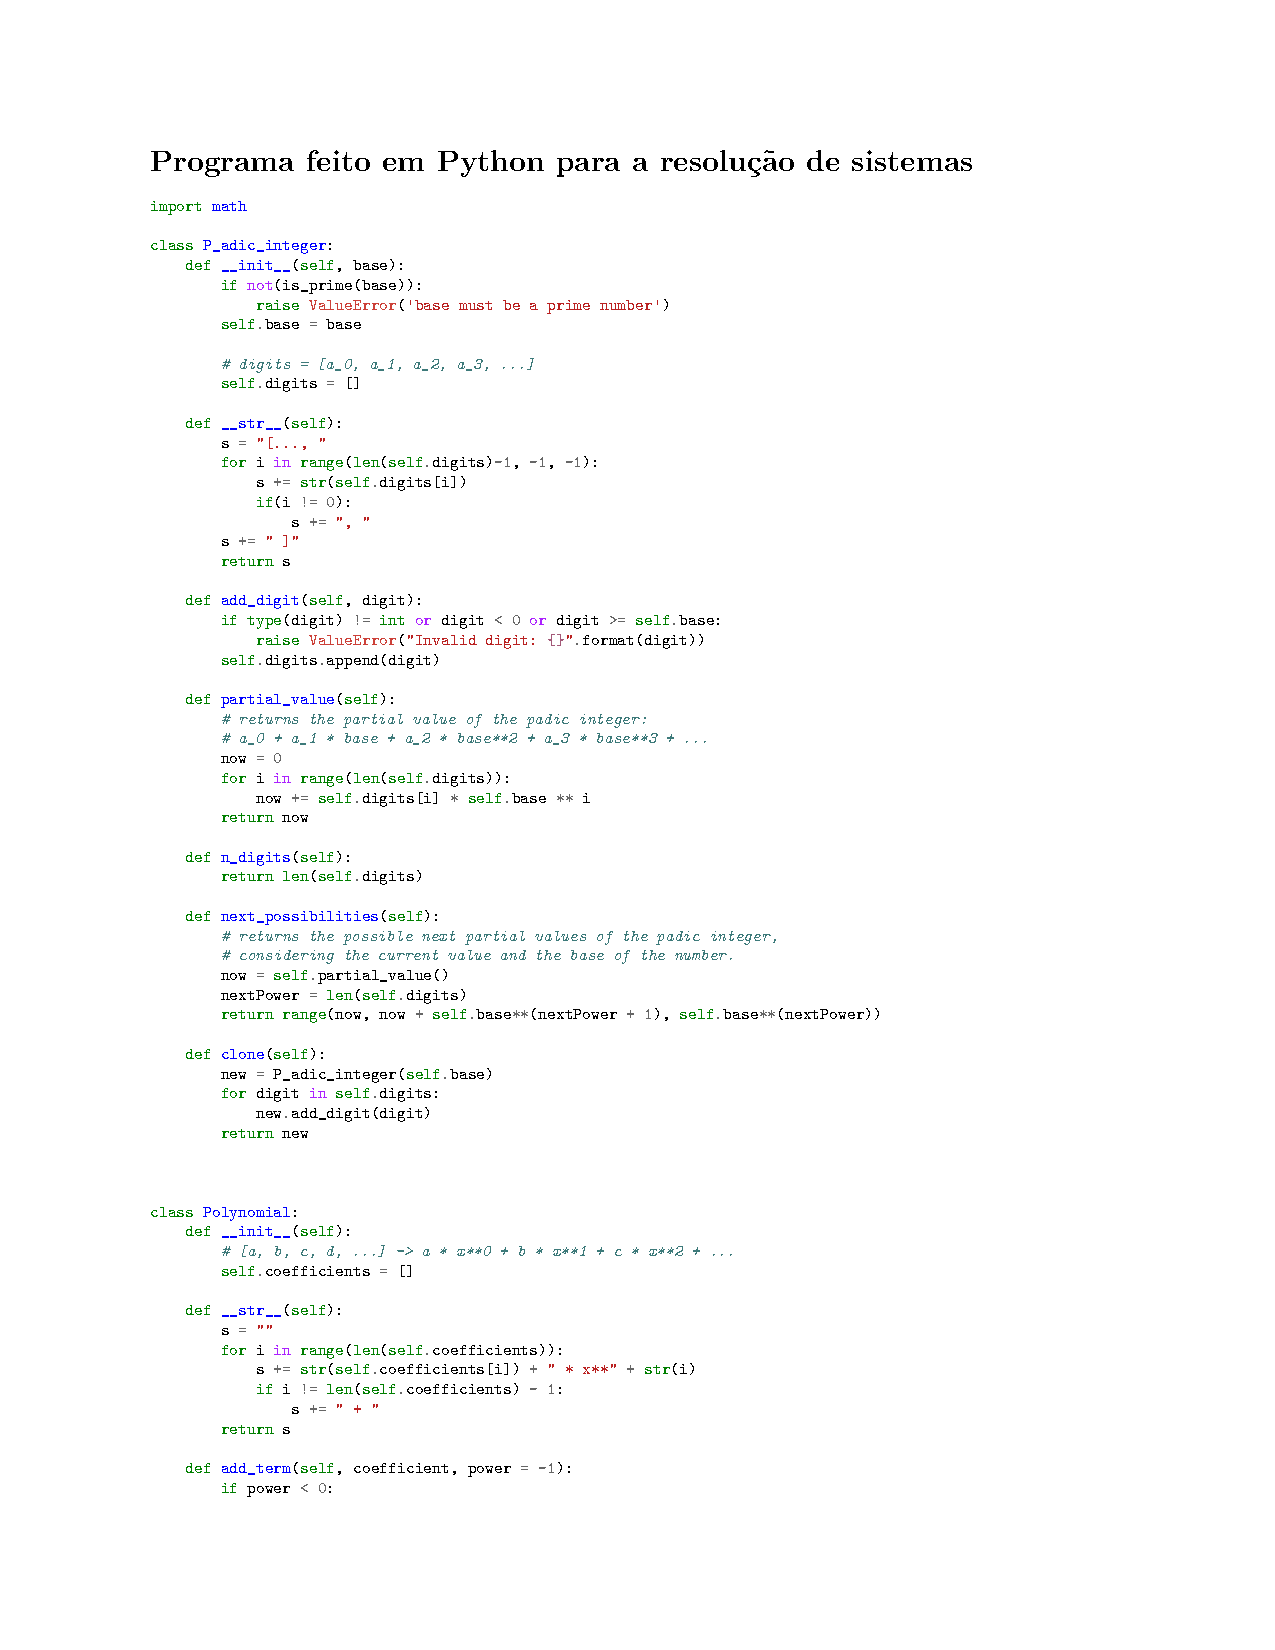
\includepdf[pages=-]{./programa/codigo.pdf}

\end{document}